
\graphicspath{{Bilder/Kap4/}}
\cleardoublepage

\chapter{Systementwurf und Umsetzung}
\label{ch:Systementwurf}
Kapitel~\ref{ch:Kapt3} hat die Anforderungen festgelegt und das Konzept mit zwei Lokalisierungsebenen ausgewählt. In diesem Kapitel wird daraus ein konkretes System. Jeder Abschnitt beschreibt zuerst das methodische Vorgehen und danach, wie es umgesetzt wurde.

Abschnitt~\ref{sec:gesamtarchitektur} gibt einen Überblick über die Komponenten und den Gesamtablauf. Abschnitt~\ref{sec:hardwareauslegung} legt Kameras, Recheneinheiten sowie die Mechanik aus. Abschnitt~\ref{sec:bildverarbeitung} beschreibt, wie aus einem Kamerabild die Pose eines Moduls entsteht, und Abschnitt~\ref{sec:servoing}, wie der Roboter die Handkamera dafür gezielt ausrichtet. Abschnitt~\ref{sec:communikation_intergration} zeigt, wie die Komponenten miteinander kommunizieren, und Abschnitt~\ref{sec:digitaler_zwilling}, wie die Ergebnisse in den digitalen Zwilling gelangen.

\section{Gesamtarchitektur}
\label{sec:gesamtarchitektur}
Die Gesamtarchitektur baut auf zwei Grundlagen auf. Die erste ist das in Kapitel~\ref{ch:Kapt3} gewählte Konzept mit mehreren Lokalisierungsebenen. Die zweite ist die vorhandene Infrastruktur des Instituts (Abschnitt~\ref{sec:Erfassen externer Randbedingungen}), der digitale Zwilling im Web-Frontend, das zugehörige Backend und OPC UA als Kommunikationsstandard. Das neue System soll sich in diese Umgebung einfügen und sie nicht ersetzen. Daraus ergeben sich fünf Entwurfsprinzipien.

\begin{itemize}
    \item \textbf{Zwei Ebenen.} Die Deckenkamera (Layer~1) erfasst den ganzen Arbeitsbereich und liefert grobe Posen aller Module. Diese Posen sind die Startwerte für die Handkamera am Roboter (Layer~2). Sie misst jedes Modul aus der Nähe nach und liefert die geforderte Genauigkeit.
    \item \textbf{Dezentrale Bildverarbeitung.} Jede Kamera hat einen eigenen Rechner, der die Bilder direkt vor Ort auswertet. Über das Netzwerk gehen nur die Ergebnisse, also wenige Zahlenwerte statt ganzer Bilder. Das hält die Netzlast gering und die Schnittstellen kompakt \cite{Shi2016}.
    \item \textbf{Einheitliche Schnittstellen.} Alle Geräte sprechen OPC UA. Ein neues Gerät mit derselben Schnittstelle lässt sich ohne Änderungen am übrigen System einbinden.
    \item \textbf{Human-in-the-loop.} Gemessene Posen sind zunächst nur Vorschläge. Der Bediener prüft sie, bevor sie in den digitalen Zwilling übernommen werden. Vor jeder Roboterbewegung stellt er außerdem sicher, dass weder Personen noch Gegenstände im Weg sind.
    \item \textbf{Gemeinsame Referenz.} Einige fest montierte und eingemessene Tags, die WorldTags, legen das Weltkoordinatensystem fest. Jede Kamera bestimmt ihre eigene Lage an diesen Tagsn. So lassen sich weitere Kameras, Roboter und damit ein größerer Arbeitsbereich ergänzen, ohne das Bezugssystem neu festzulegen.
\end{itemize}

Aus diesen Prinzipien leiten sich die in Abbildung~\ref{fig:komponentendiagramm} gezeigten Komponenten ab. Die AprilTags teilen sich in WorldTags und ModulTags. WorldTags sind ortsfest und eingemessen, während ModulTags an den Modulen sitzen und sich mit ihnen bewegen. Ein Modul kann dabei mehrere ModulTags tragen, sodass wenn Tags verdeckt ist oder der Roboter ihn mit der Handkamera nicht erreichen kann, das Modul über einen anderen Tag bestimmt wird. Da die relative Lage jedes Tags am Modul bekannt ist, führt jeder von ihnen zur selben Modulpose. Diese werden von der Deckenkamera sowie der am Roboterflansch montierten Handkamera erfasst. Beide Kameras sind jeweils mit einem eigenen Raspberry Pi verbunden und laufen mit demselben Programm. Das Programm detektiert die Tags, berechnet deren Pose und stellt die Ergebnisse über einen OPC-UA-Server zur Verfügung. Welche Rolle ein Pi übernimmt, legt allein seine Konfiguration fest. Die Wahl der Hardware wird in Abschnitt~\ref{sec:hardwareauslegung} begründet.

Das bestehende Backend dient als Gateway. Es verbindet sich als OPC-UA-Client mit beiden Pis und mit dem Roboter und und leitet die Messergebnisse und Statusmeldungen an den digitalen Zwilling im Browser weiter. Dort liegen die 3D-Szene, der Modulkatalog und die Posenplanung. Der Modulkatalog beschreibt jedes Modul, das das System kennt. Dort werden die Abmessungen, das 3D-Modell und die Position der Tags am Modul hinterlegt. Ein Tag trägt also nur eine ID, seine Bedeutung ergibt sich erst aus dem Katalog (siehe Abschnitt~\ref{sec:digitaler_zwilling}). Kurz gesagt messen die Pis, plant der digitale Zwilling und das Backend vermittelt. Der gestrichelt dargestellte Videostream dient lediglich der Anzeige und ist nicht Teil des Messablaufs (siehe Abschnitt~\ref{sec:communikation_intergration}).
% SVEN (Notiz zu "leitet die empfangenen Daten"): Hier nur die Bilder nicht alle daten das ist im Schaubild gut gezeigt


\begin{figure}[htbp]
    \centering
    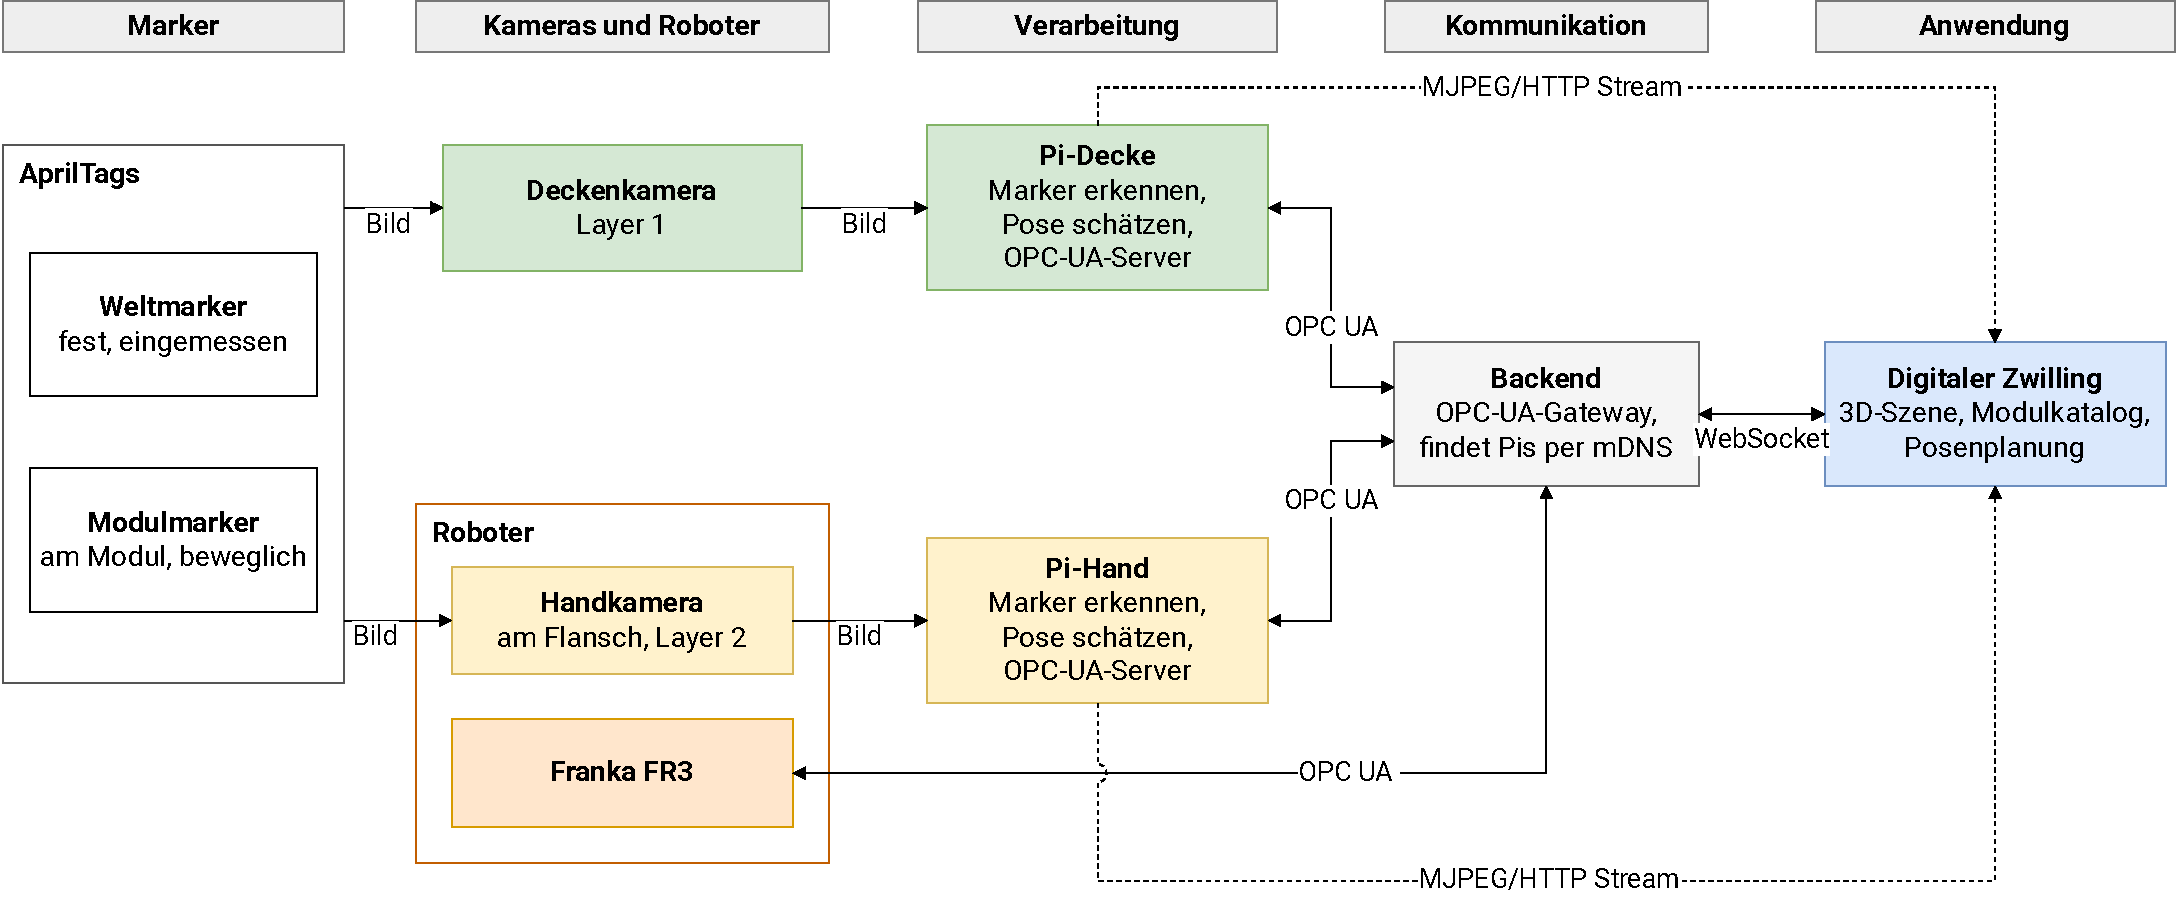
\includegraphics[width=\textwidth]{01_Komponentendiagramm_v2.pdf}
    \caption{Komponentendiagramm des Gesamtsystems. Die gestrichelte Linie stellt den optionalen Videostream der Kameras dar.}
    \label{fig:komponentendiagramm}
\end{figure}

Wie die Komponenten zusammenarbeiten, zeigt der Gesamtablauf in Abbildung~\ref{fig:gesamtablauf}. Jede Spalte steht für eine Komponente. Alle Nachrichten zwischen den Spalten laufen über das Backend. Die verwendeten Symbole erklärt Abbildung~\ref{fig:legende}.

Zu Beginn legt der Bediener im Frontend die Zellkarte an. Diese enthält die WorldTags sowie den Katalog der Module inklusive ihrer Tags. Parallel dazu erkennt das Backend die gestarteten Raspberry Pis selbstständig im Netzwerk. Danach prüft jeder Pi, ob für seine Kamera eine passende Kalibrierung vorliegt. Fehlt sie oder passt sie nicht zur eingestellten Auflösung, wird die Kamera mithilfe des Roboters neu kalibriert (Abschnitt~\ref{sec:bildverarbeitung}).

Anschließend startet der Bediener den Layer-1-Scan. Der Decken-Pi nimmt den Arbeitsbereich auf und schickt die Posen der erkannten Tags zurück. Das Frontend lädt damit die Module in die 3D-Szene. Diese groben Posen sind der Ausgangspunkt für alle weiteren Schritte.

Auf Grundlage der Szene plant das Frontend die Messfahrt für Layer~2. Gleichzeitig übernimmt es über die Funktionen Take Control und Sync die Kontrolle über den Roboter. Bei der Messfahrt fährt der Roboter nacheinander Sichtpunkte, startenden bei einem WorldTag vor den Modulen an. An jedem Sichtpunkt misst der Hand-Pi die Tags und gibt die Messwerte zurück. Wie sich der Roboter dabei auf den Tags ausrichtet, beschreibt Abschnitt~\ref{sec:servoing}.

Aus den Messwerten entsteht ein Vorschlag mit präzisen Posen. Der Bediener entscheidet, ob er ihn übernimmt. Lehnt er ab, bleiben die Posen aus Layer~1 erhalten. Der digitale Zwilling bleibt also in jedem Fall in einem gültigen Zustand.

Zum Schluss startet die Zellüberwachung auf dem Decken-Pi. Sie vergleicht laufend die erkannten Posen mit dem Stand im digitalen Zwilling. Wird ein Modul um \SI{15}{\centi\metre} oder mehr verschoben, beginnt der Ablauf mit einem neuen Scan von vorn. Kleinere Abweichungen lösen keinen neuen Scan aus.

% Kompakte Legende der Ablaufdiagramme, nachgezeichnet nach 00_Legende_v3 (draw.io).
% Erstellt mit Claude Opus 5.5, siehe KI-Hilfsmittel-Verzeichnis.
\begin{figure}[htbp]
    \centering
    \footnotesize
    \newcommand{\legsym}[1]{\tikz[baseline=0.07cm, line width=0.4pt, x=1cm, y=1cm]{#1}}
    \begin{tabular}{@{}c@{\hspace{0.5em}}l@{\hspace{1.5em}}c@{\hspace{0.5em}}l@{}}
        \legsym{\draw[rounded corners=0.18cm] (0,0) rectangle (1,0.36);} & Start / Ende
        & \legsym{\draw (0,0) rectangle (1,0.36); \draw (0.1,0) -- (0.1,0.36); \draw (0.9,0) -- (0.9,0.36);} & Unterprozess (eigene Abbildung) \\[0.6ex]
        \legsym{\draw (0,0) rectangle (1,0.36);} & Prozessschritt
        & \legsym{\draw (0,0.36) -- (1,0.36) -- (0.86,0) -- (0.14,0) -- cycle;} & Bedienung im Frontend \\[0.6ex]
        \legsym{\draw (0,0.18) -- (0.5,0.38) -- (1,0.18) -- (0.5,-0.02) -- cycle;} & Entscheidung (ja/nein)
        & \legsym{\draw (0,0.18) -- (0.18,0.36) -- (0.82,0.36) arc (90:-90:0.18) -- (0.18,0) -- cycle;} & Anzeige (3D-Szene) \\[0.6ex]
        \legsym{\draw[densely dashed] (0,0.18) -- (0.5,0.38) -- (1,0.18) -- (0.5,-0.02) -- cycle;} & Vereinfacht, nicht im Projektumfang
        & \legsym{\draw[line width=0.8pt] (0,0.23) -- (1,0.23); \draw[line width=0.8pt] (0,0.13) -- (1,0.13);} & Parallele Abläufe beginnen/enden \\[0.8ex]
        \multicolumn{4}{@{}l@{}}{\glqq via Backend\grqq: Aufruf bzw. Daten laufen über das Backend (OPC-UA-Gateway).}
    \end{tabular}
    \caption[Legende der Ablaufdiagramme]{Legende der Ablaufdiagramme in diesem Kapitel. Erstellt mit dem KI-Hilfsmittel Claude Opus 5.5 (Anthropic), siehe KI-Hilfsmittel-Verzeichnis.}
    \label{fig:legende}
\end{figure}

\begin{figure}[htbp]
    \centering
    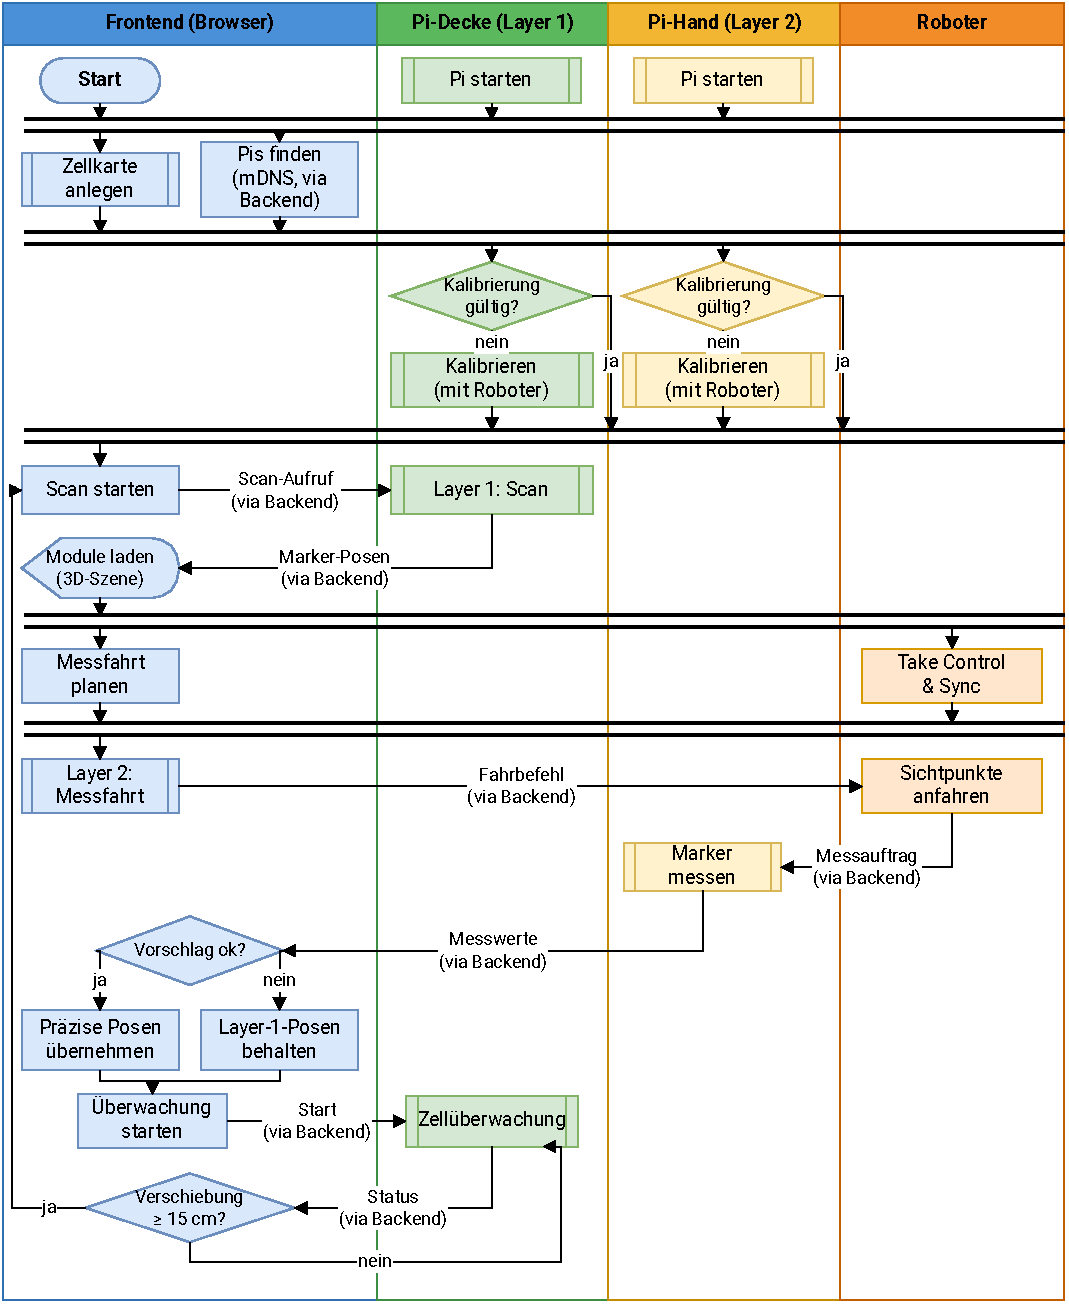
\includegraphics[width=\textwidth]{02_Gesamtablauf_v3.pdf}
    \caption{Gesamtablauf der Lokalisierung, aufgeteilt auf Frontend, Decken-Pi, Hand-Pi und Roboter. Alle Nachrichten zwischen den Komponenten laufen über das Backend. Überarbeite ich nochmal final. Mit Querverweisen auf die anderen Diagrammen und Pseudocode aus dem Kapitel}
    \label{fig:gesamtablauf}
\end{figure}

% -----------------------------------------------------------------------------
% Abschnitte 4.2 bis 4.4: Entwurf erstellt mit Claude Opus 5.5 (Anthropic) aus
% Folien, Code und Projektdoku, siehe KI-Hilfsmittel-Verzeichnis.
% Offene Stellen sind mit \Add{[OFFEN: ...]} markiert.
% -----------------------------------------------------------------------------
\section{Hardwareauslegung}
\label{sec:hardwareauslegung}
Die Hardware muss das Konzept aus Kapitel~\ref{ch:Kapt3} tragen. Die Deckenkamera soll den Arbeitsbereich von \qtyproduct{2 x 2}{\metre} vollständig sehen (A1). Die Handkamera soll die Module so genau messen, dass die Positioniergenauigkeit von \SI{\pm 3}{\milli\metre} erreichbar ist (A3). Die Kosten dürfen \SI{1000}{\euro} nicht überschreiten, vorhandenes Material ist zu bevorzugen (A2), und kein Aufbau darf Personen gefährden (A6). Dieser Abschnitt legt nacheinander die Deckenkamera, die Handkamera, die Recheneinheiten, die Halterung der Deckenkamera und die Tags aus.

\subsection{Deckenkamera}
\label{subsec:hw-deckenkamera}
Bei der Deckenkamera stehen zwei Ziele gegeneinander. Eine kurze Brennweite vergrößert das Bildfeld, bildet einen Tag aber kleiner ab. Eine lange Brennweite bewirkt das Gegenteil. Gesucht ist deshalb ein Bereich von Abständen, in dem beide Ziele erfüllt sind. Ausgelegt wurde auf Tags mit \SI{75}{\milli\metre} Kantenlänge, die mit mindestens 80~Pixeln je Kante abgebildet werden sollen. \Add{[OFFEN: Herkunft der 80 Pixel]}

Damit der Arbeitsbereich mit der Breite $b$ auf die kurze Sensorseite passt, muss die Kamera mindestens den Abstand
\begin{equation}
    d_{\min} = \frac{f \cdot b}{n_{\mathrm{kurz}} \cdot p}
    \label{eq:hw-dmin}
\end{equation}
haben. Dabei ist $f$ die Brennweite, $n_{\mathrm{kurz}}$ die Pixelzahl der kurzen Sensorseite und $p$ der Pixelabstand. Damit ein Tag der Kantenlänge $s$ noch mit $n_{\mathrm{Tag}}$ Pixeln abgebildet wird, darf die Kamera höchstens
\begin{equation}
    d_{\max} = \frac{f \cdot s}{n_{\mathrm{Tag}} \cdot p}
    \label{eq:hw-dmax}
\end{equation}
vom Tag entfernt sein. Eine Kombination aus Kamera und Objektiv ist geeignet, wenn der Abstand zwischen Kamera und Tag-Ebene in diesem Bereich liegt und die Kamera dort auch montiert werden kann.

Außerdem muss das Bild im ganzen Bereich scharf sein. Die Schärfentiefe folgt aus der hyperfokalen Distanz $H$:
\begin{equation}
    H = f + \frac{f^2}{N \cdot c},
    \qquad
    d_{\mathrm{nah}} = \frac{H \cdot d}{H + (d - f)},
    \qquad
    d_{\mathrm{fern}} = \frac{H \cdot d}{H - (d - f)} .
    \label{eq:hw-schaerfe}
\end{equation}
Dabei ist $N$ die Blendenzahl, $d$ der Fokusabstand und $c$ der zulässige Zerstreuungskreis. Für $c$ wurde der doppelte Pixelabstand angesetzt. An einer Kante zwischen Schwarz und Weiß darf ein Pixel damit in den Nachbarn übergehen, aber nicht weiter. Schließlich muss jede Zelle des Tag-Musters nach dem Abtasttheorem mindestens ein Pixel breit abgebildet werden:
\begin{equation}
    \frac{1}{2\,g_{\mathrm{Sensor}}} \le \frac{1}{2\,p}
    \quad\Longleftrightarrow\quad
    g_{\mathrm{Sensor}} = \frac{g \cdot f}{d} \ge p ,
    \label{eq:hw-nyquist}
\end{equation}
mit der Zellgröße $g$ auf dem Tag und $g_{\mathrm{Sensor}}$ auf dem Sensor. Bei 80~Pixeln je Kante und acht Zellen über das schwarze Quadrat entfallen etwa zehn Pixel auf eine Zelle. Diese Bedingung ist damit weit erfüllt, maßgebend bleibt Gleichung~\eqref{eq:hw-dmax}.

Tabelle~\ref{tab:hw-kamerawahl} vergleicht die betrachteten Kameras. Unter der Hallendecke liegen in \SI{3,70}{\metre} Höhe Deckenpaneele und in \SI{3,00}{\metre} Höhe Lampen. Bei Tags in \SI{1,0}{\metre} Höhe bleibt damit ein Abstand von höchstens etwa \SI{2}{\metre}. Die Camera Module~3 mit fester Brennweite und die HQ Camera mit \SI{6}{\milli\metre}-Objektiv müssten über den Lampen hängen. Die Industriekamera wäre geeignet, kostet aber etwa das Achtfache der HQ Camera. Ihr größerer Pixelabstand verbessert zwar das Signal-Rausch-Verhältnis, bei den großen, kontrastreichen Flächen eines AprilTags bringt das jedoch wenig.

\begin{table}[htbp]
    \centering
    \caption{Betrachtete Deckenkameras (Arbeitsbereich \SI{2}{\metre}, Tag \SI{75}{\milli\metre}, 80~Pixel)}
    \label{tab:hw-kamerawahl}
    \small
    \begin{tabular}{lrrrrr}
        \toprule
        \textbf{Kamera} & \textbf{Preis} & \textbf{Sensor (Pixel)} & \textbf{$p$} & \textbf{$f$} & \textbf{$d_{\min}$ bis $d_{\max}$} \\
        \midrule
        RPi Camera Module~3 & \SI{29,90}{\euro} & \numproduct{4608 x 2592} & \SI{1,40}{\micro\metre} & \SI{4,75}{\milli\metre} & \SIrange{2,62}{3,17}{\metre} \\
        RPi HQ Camera, M12  & \SI{55,45}{\euro} & \numproduct{4056 x 3040} & \SI{1,55}{\micro\metre} & \SI{6}{\milli\metre}    & \SIrange{2,54}{3,62}{\metre} \\
        RPi HQ Camera, M12  & \SI{55,45}{\euro} & \numproduct{4056 x 3040} & \SI{1,55}{\micro\metre} & \SI{2,7}{\milli\metre}  & \SIrange{1,14}{1,63}{\metre} \\
        Industriekamera \Add{[OFFEN: Modell]} & \SI{679}{\euro} & \numproduct{5472 x 3648} & \SI{2,40}{\micro\metre} & \SI{6}{\milli\metre} & \SIrange{1,37}{2,34}{\metre} \\
        \bottomrule
    \end{tabular}
\end{table}

Gewählt wurde die Raspberry Pi HQ Camera (Sensor IMX477) mit einem M12-Weitwinkelobjektiv von \SI{2,7}{\milli\metre} Brennweite und einem Bildwinkel von etwa \qtyproduct{99 x 82}{\degree}. Abbildung~\ref{fig:hw-kamera-auslegung} zeigt die Auslegung. In \SI{2,63}{\metre} Höhe und mit Fokus auf \SI{1,5}{\metre} ist das Bild bei Blende~1,0 von \SIrange{0,91}{4,12}{\metre} scharf ($H = \SI{2,35}{\metre}$). Tische und Boden liegen damit vollständig im scharfen Bereich. Am Boden deckt die kurze Bildseite \SI{4,60}{\metre} ab.

\begin{figure}[htbp]
    \centering
    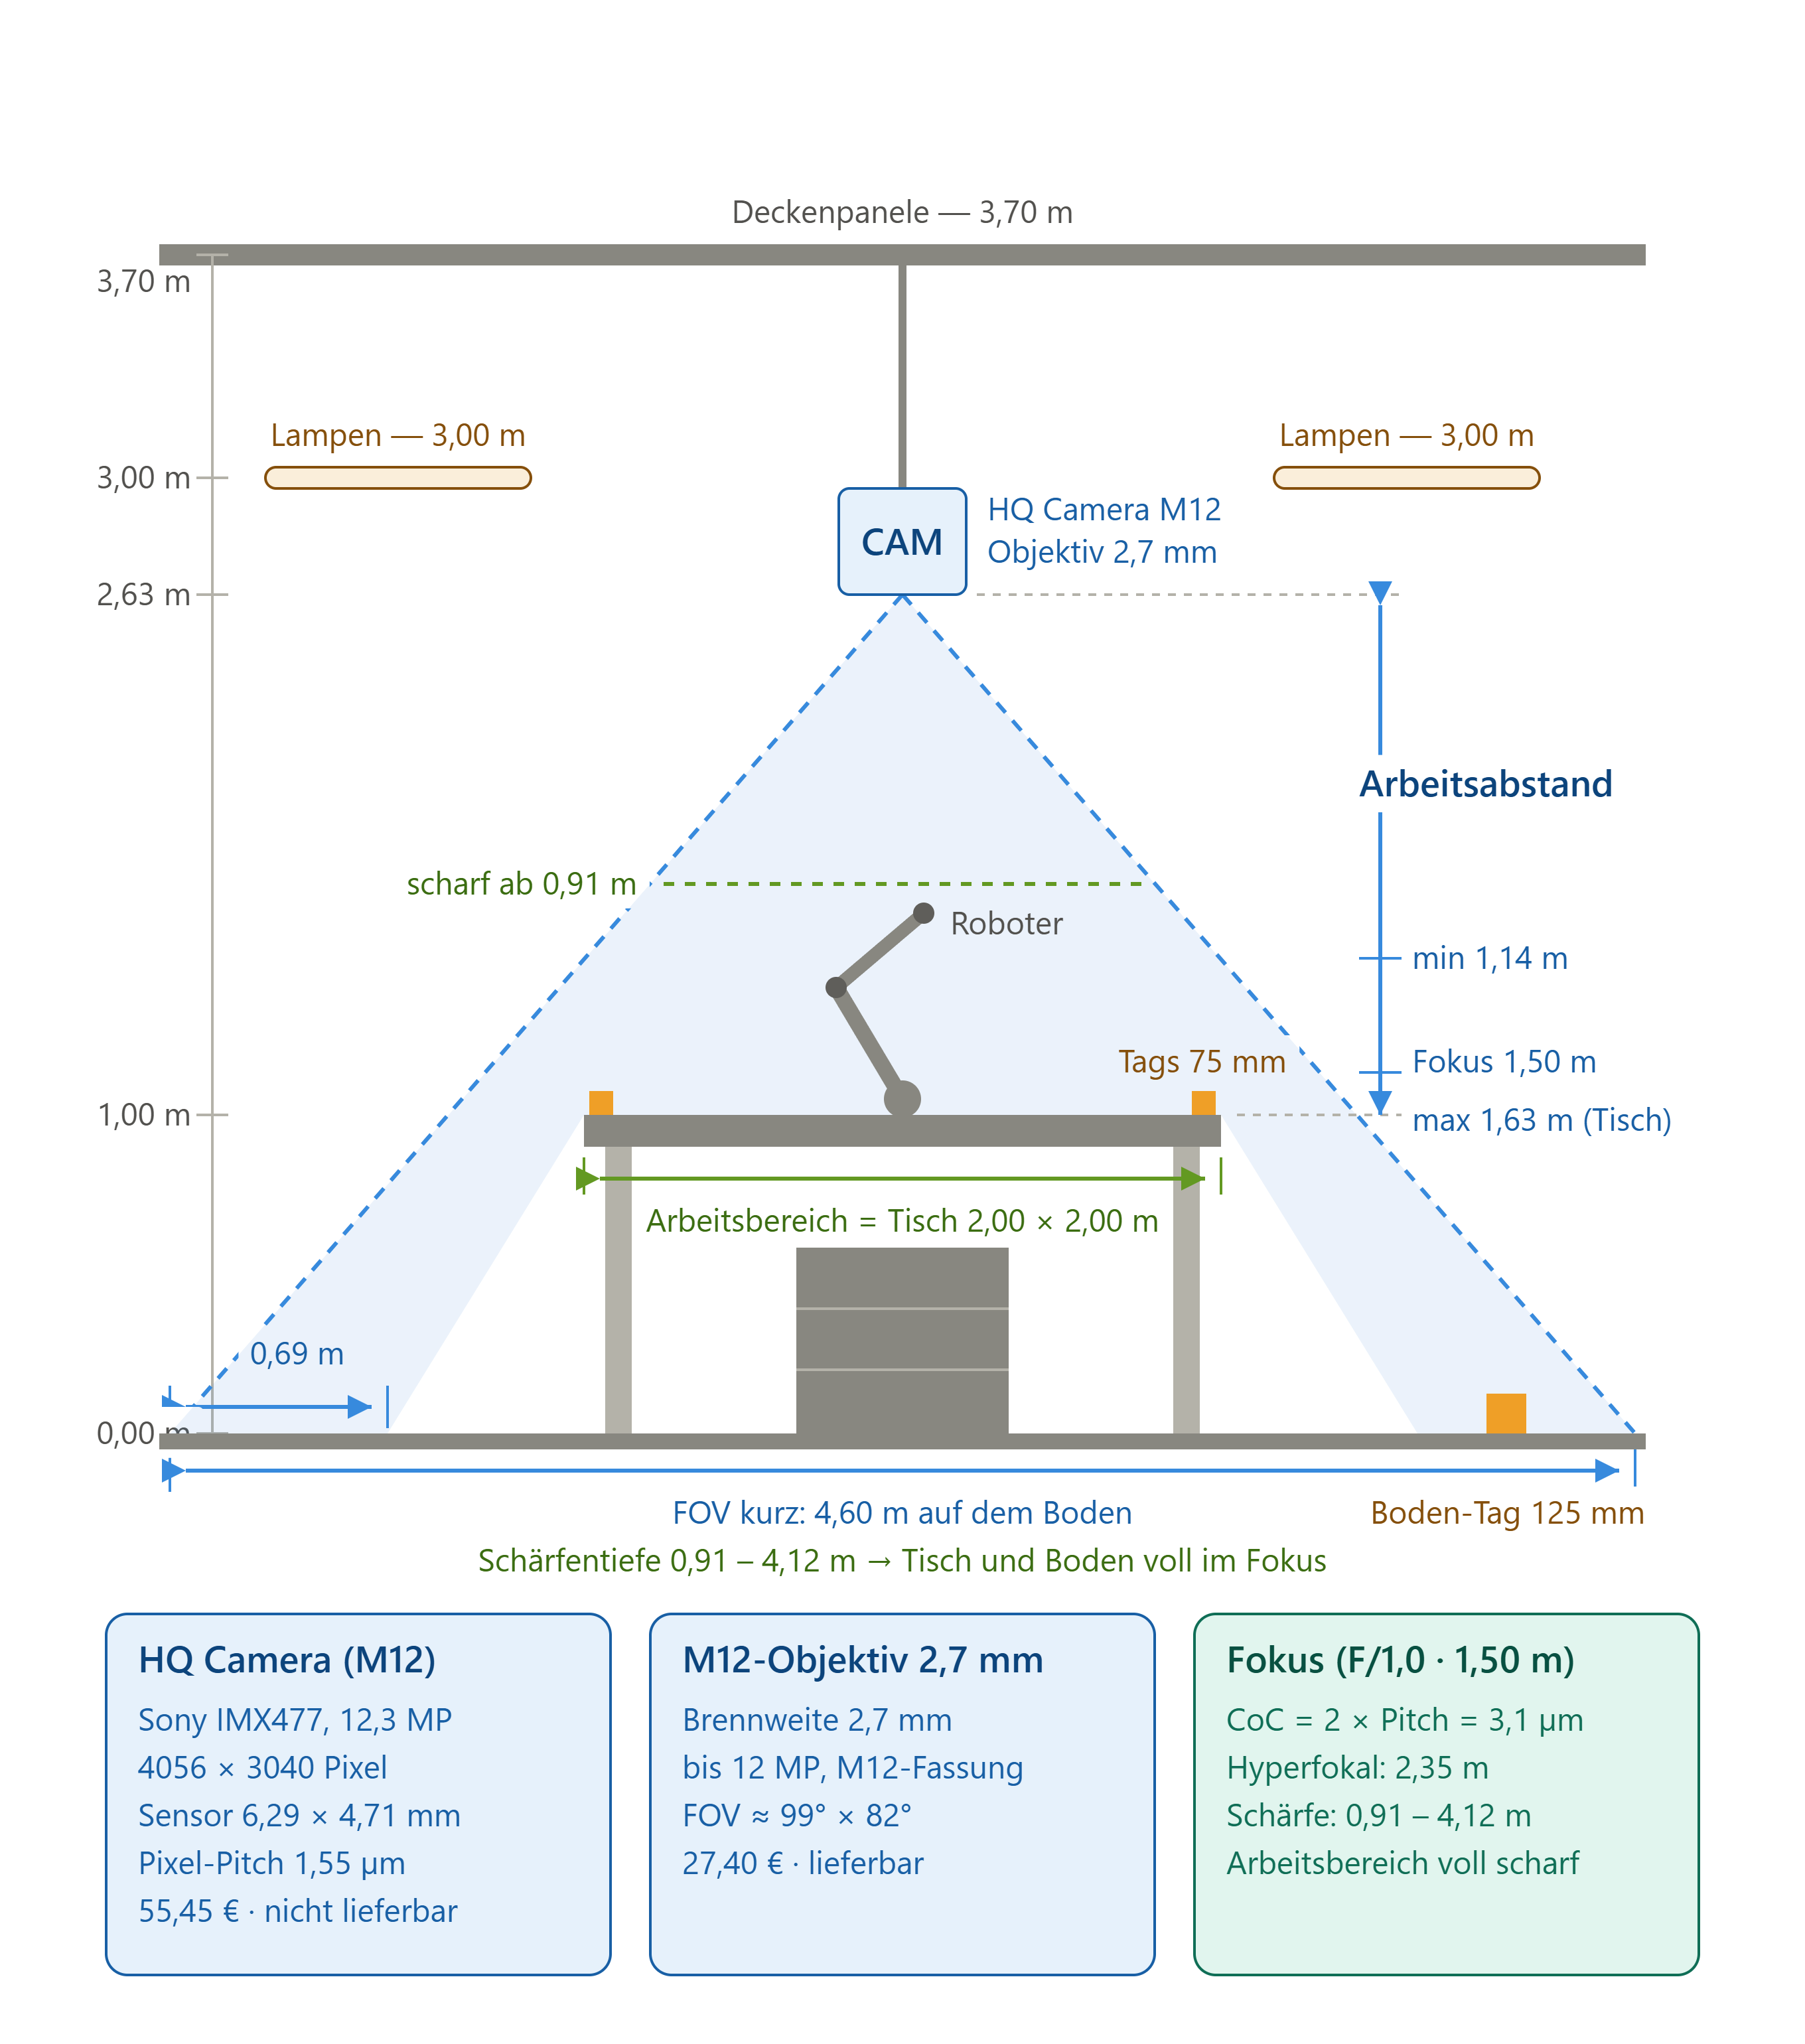
\includegraphics[width=0.75\textwidth]{20_Kamera_Auslegung.png}
    \caption{Auslegung der Deckenkamera mit Arbeitsabstand und Schärfentiefe (Konzeptwerte: Tags \SI{75}{\milli\metre}, Boden-Tag \SI{125}{\milli\metre})}
    \label{fig:hw-kamera-auslegung}
\end{figure}

Das M12-Objektiv hat keine Blende. Einstellbar ist nur der Fokus, indem das Objektiv im Gewinde gedreht wird. Er ist auf die Bodenebene eingestellt (Abschnitt~\ref{subsec:bv-layer1}). Ein ModulTag wird damit mit etwa 85~Pixeln Kantenlänge abgebildet, also über dem Auslegungsziel. \Add{[OFFEN: tatsächliche Montagehöhe der Kamera]}

\subsection{Handkamera}
\label{subsec:hw-handkamera}
Die Handkamera misst einzelne Tags aus etwa \SIrange{14}{35}{\centi\metre} Entfernung (Abschnitt~\ref{sec:servoing}). Ein Tag füllt dort einen großen Teil des Bildes, sodass eine geringe Auflösung genügt. Eingesetzt wird eine Intel RealSense, von der nur das Farbbild mit \numproduct{640 x 480} Pixeln genutzt wird. \Add{[OFFEN: Modell der RealSense; Grund der Wahl, z.\,B. bereits vorhanden (A2); warum das Tiefenbild nicht genutzt wird]}

Die Kamera sitzt über einen Halter am Werkzeugflansch des Roboters. Gegenüber einer zweiten fest montierten Kamera hat diese Anordnung den Vorteil, dass die Kamera jedes Modul aus kurzer Entfernung und aus mehreren Richtungen sehen kann. Die Lage der Kamera am Flansch wird einmal kalibriert (Abschnitt~\ref{subsec:bv-kalibrierung}). Laut dieser Kalibrierung liegt das optische Zentrum etwa \SI{47}{\milli\metre}, \SI{35}{\milli\metre} und \SI{61}{\milli\metre} in $x$, $y$ und $z$ vom Flansch entfernt. Die Kalibrierung bleibt nur gültig, solange der Halter steif ist und nicht kriecht. \Add{[OFFEN: Halter -- Bauform, Werkstoff, Fertigung, Foto]}

Kunststoffe aus dem 3D-Drucker kriechen unter Dauerlast, wobei die Spannung stärker wirkt als die Temperatur. PLA verformt sich bei \SI{25}{\degreeCelsius} und \SI{20}{\mega\pascal} in drei Stunden um etwa \SI{290}{\micro\metre}, bei \SI{40}{\degreeCelsius} um etwa \SI{1850}{\micro\metre}. Für dauerhaft belastete Teile eignen sich PC, CPE und ABS deutlich besser \tocite{Dogan 2022, Kriechverhalten 3D-gedruckter Kunststoffe}. Die Rangfolge steht in Anhang~\ref{app:Mechanik}. \Add{[OFFEN: welche Teile gedruckt wurden und aus welchem Werkstoff]}

\subsection{Recheneinheiten}
\label{subsec:hw-rechner}
Die Recheneinheit wurde über eine Nutzwertanalyse ausgewählt (Tabelle~\ref{tab:hw-nwa-rechner}). Der Raspberry Pi liegt vorn: Er verarbeitet AprilTags schnell genug, ist günstig und lässt sich direkt an der Kamera montieren. Ein Jetson Orin Nano wäre nur dann im Vorteil, wenn KI-Verfahren wie YOLO hinzukommen.

\begin{table}[htbp]
    \centering
    \caption{Nutzwertanalyse der Recheneinheit (Bewertung von 1 bis 5)}
    \label{tab:hw-nwa-rechner}
    \begin{tabular}{lcccc}
        \toprule
        \textbf{Kriterium} & \textbf{Gewicht} & \textbf{Raspberry Pi 5} & \textbf{Jetson Orin Nano} & \textbf{Industrie-PC} \\
        \midrule
        AprilTag-Verarbeitung     & \num{0,25} & 4 & 5 & 5 \\
        Erweiterbarkeit KI / YOLO & \num{0,15} & 2 & 5 & 4 \\
        Kosten                    & \num{0,35} & 5 & 3 & 1 \\
        Formfaktor / Montage      & \num{0,25} & 5 & 4 & 2 \\
        \midrule
        \textbf{Gewichteter Nutzwert} & \num{1,00} & \textbf{\num{4,30}} & \num{4,05} & \num{2,70} \\
        \bottomrule
    \end{tabular}
\end{table}

An der Hand arbeitet ein Raspberry Pi~5. Beim visuellen Servoing wartet der Roboter auf jede Messung, die Rechenzeit verlängert also unmittelbar die Messfahrt. Zudem lässt der Pi~5 Raum für spätere Verfahren wie YOLO (A1). An der Decke genügt ein Raspberry Pi~4. Die Deckenkamera muss Tags zuverlässig erkennen, aber nicht schnell. Da sich die Module zwischen zwei Prozessschritten nicht bewegen, ist die Latenz hier unkritisch (A4). \Add{[OFFEN: bestätigen, dass der Pi~4 aus dem Bestand stammt (A2)]}

\subsection{Halterung der Deckenkamera}
\label{subsec:hw-halterung}
Die Deckenkamera muss etwa über der Mitte der Zelle hängen (Abbildung~\ref{fig:hw-sichtfeld}). Daraus ergeben sich mehrere Anforderungen an die Halterung. Sie darf nichts in der Zelle auf den Boden stellen, sie muss sicher halten (A5, A6), und sie wird ohne Eingriff in die Bausubstanz an einer Säule neben der Zelle befestigt. \Add{[OFFEN: bestätigen, dass in der Säule nicht gebohrt werden durfte]}

\begin{figure}[htbp]
    \centering
    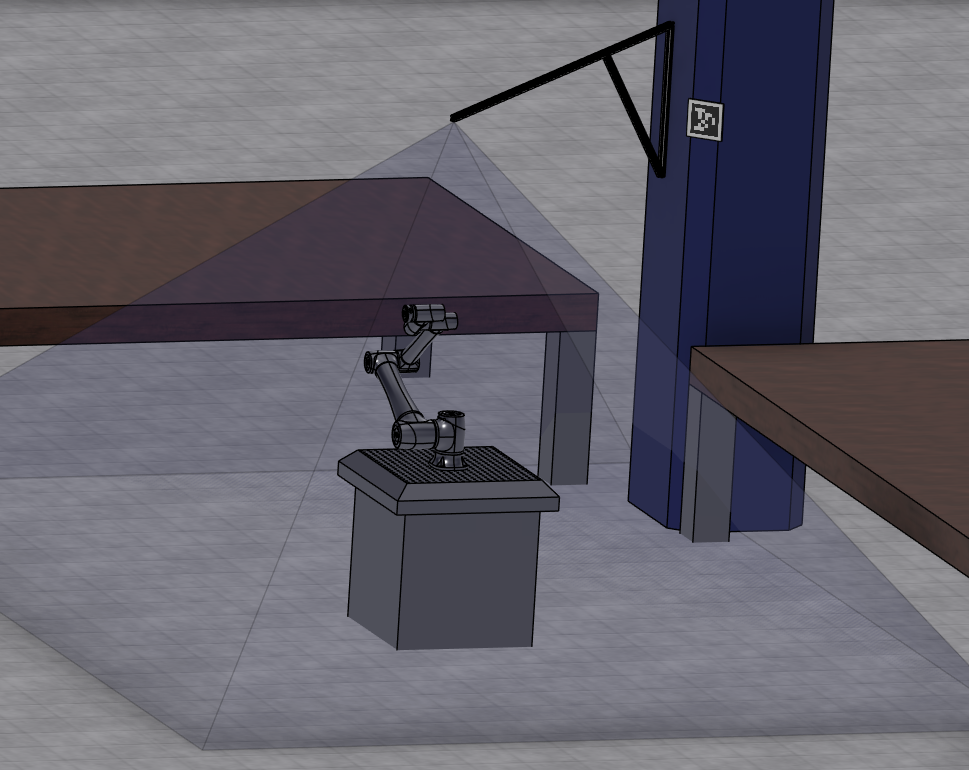
\includegraphics[width=0.55\textwidth]{21_Zelle_Sichtfeld_CAD.png}
    \caption{Konzept der Deckenkamera an einem Kragarm an der Säule mit Sichtkegel über Roboter und Tischen (CAD-Modell)}
    \label{fig:hw-sichtfeld}
\end{figure}

Betrachtet wurden drei Varianten (Abbildung~\ref{fig:hw-varianten}): ein Kragarm aus Kantholz an der Säule, ein frei stehender Galgen aus Holz und ein Kragarm aus Item-Profilen, der über eine Strebe gegen einen senkrechten Mast abgestützt ist. Für das Kantholz (\qtyproduct{8 x 8}{\centi\metre}, C24) wurde abgeschätzt, wie weit es auf \SI{3}{\metre} Ausladung durchhängt. Die Spitze senkt sich um etwa \SI{7,3}{\milli\metre}, davon \SI{7,1}{\milli\metre} durch das Eigengewicht. Die Biegespannung bleibt weit unter der Festigkeit, doch das Eigengewicht bestimmt Durchbiegung und Moment an der Säule (Anhang~\ref{app:Mechanik}). Der Galgen bräuchte zwei Stützen im Arbeitsbereich.

\begin{figure}[htbp]
    \centering
    \begin{subfigure}[b]{0.32\textwidth}
        \centering
        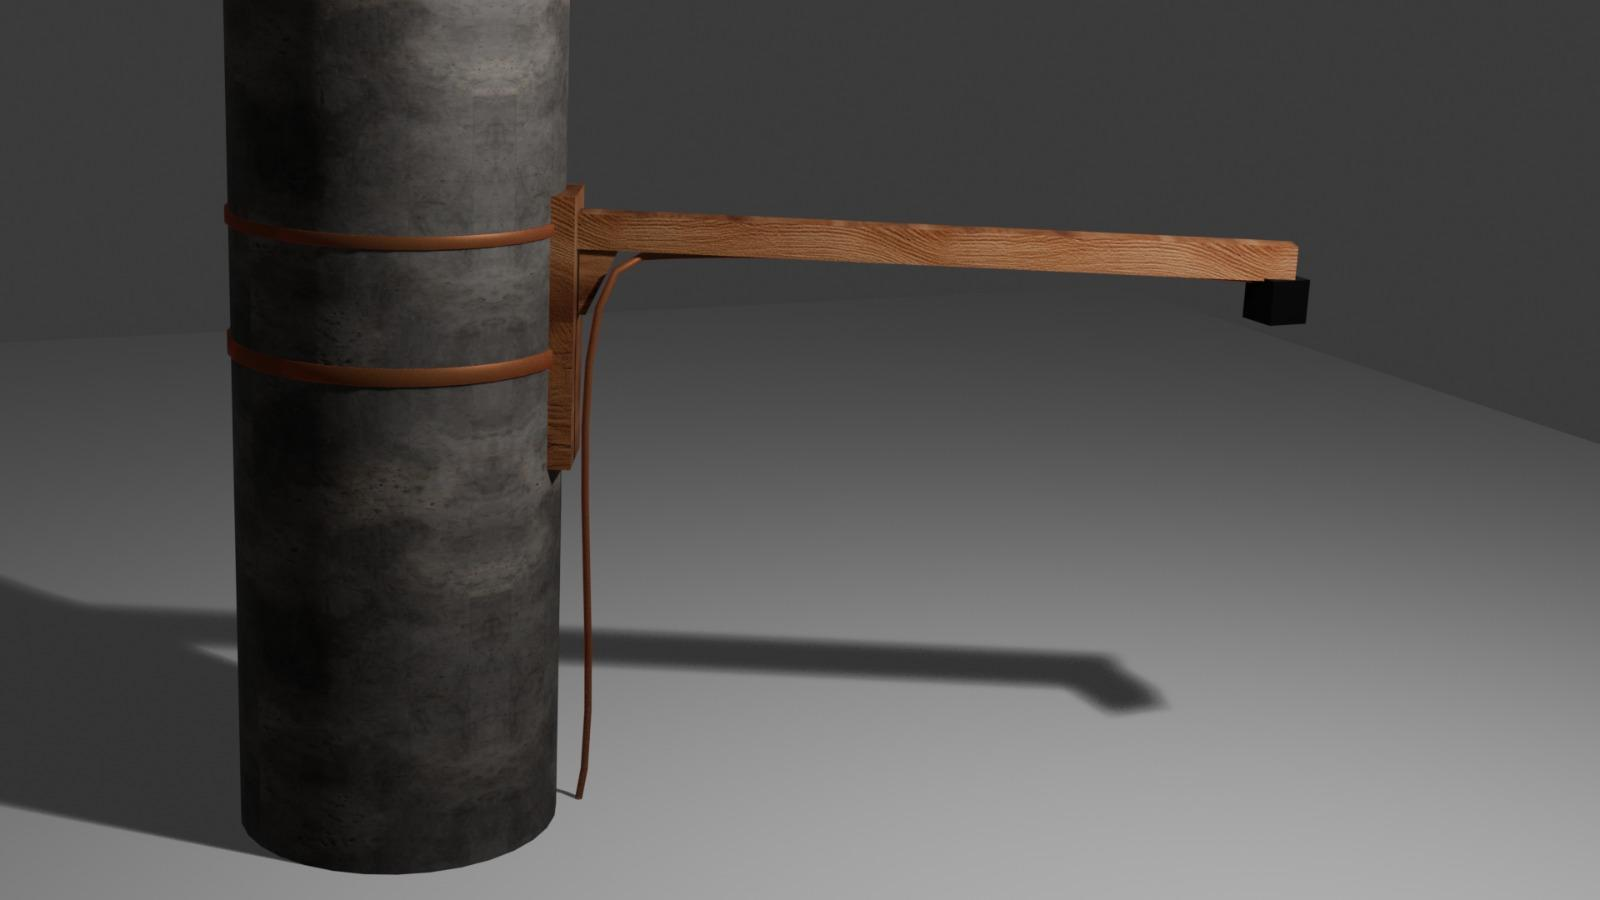
\includegraphics[width=\textwidth]{22_Halterung_Holz_Kragarm.jpg}
        \caption{Holz-Kragarm}
    \end{subfigure}\hfill
    \begin{subfigure}[b]{0.32\textwidth}
        \centering
        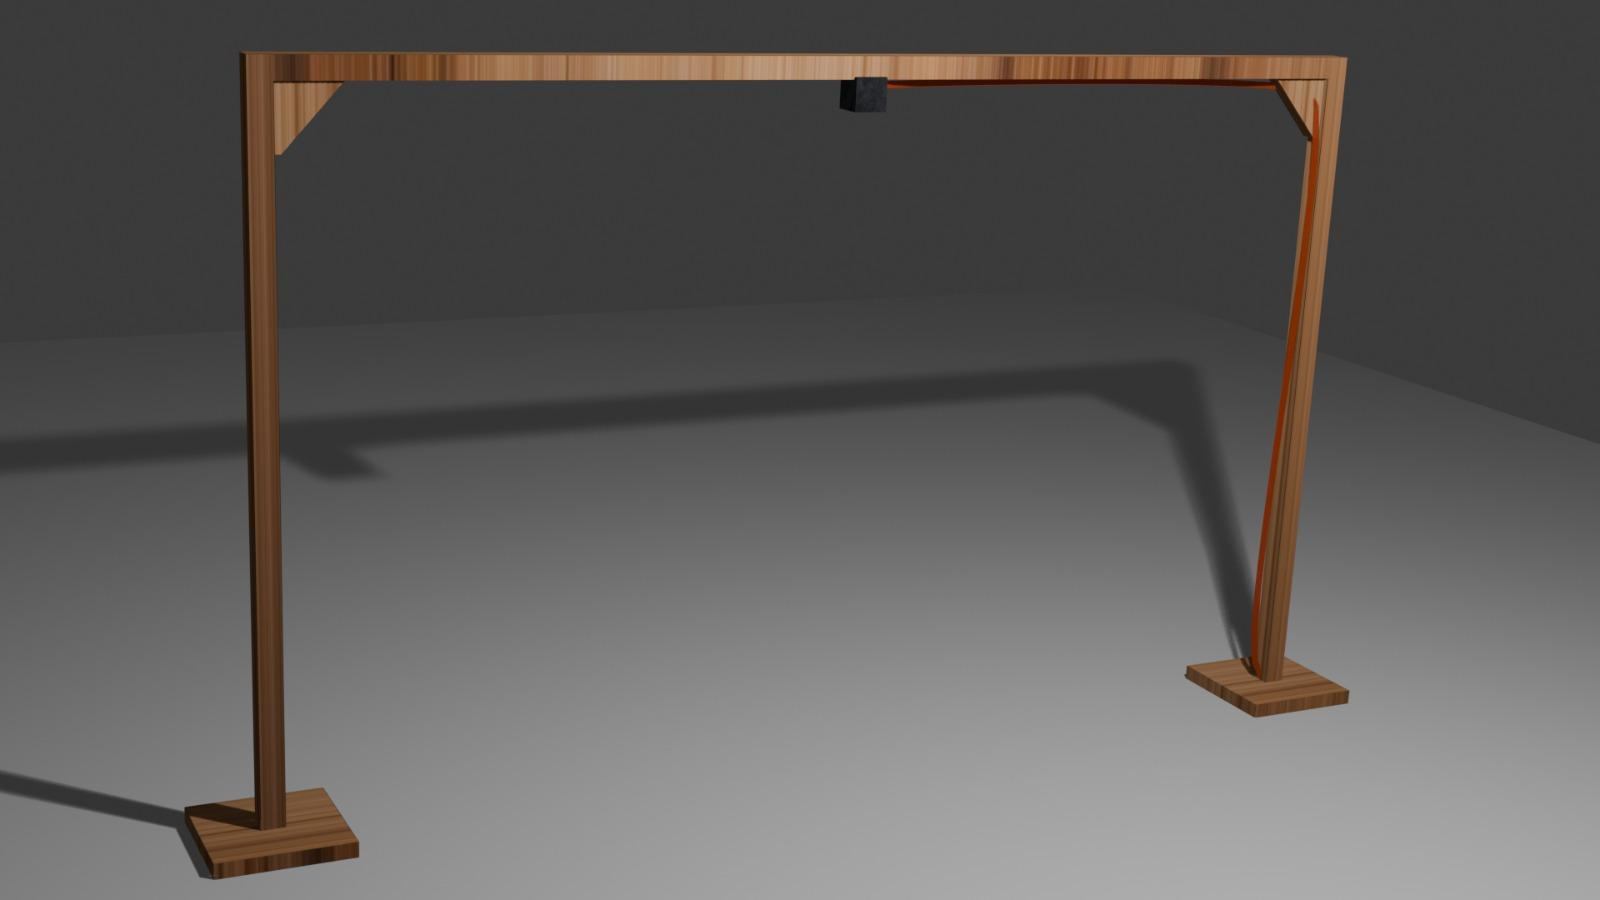
\includegraphics[width=\textwidth]{23_Halterung_Holz_Galgen.jpg}
        \caption{Holz-Galgen}
    \end{subfigure}\hfill
    \begin{subfigure}[b]{0.32\textwidth}
        \centering
        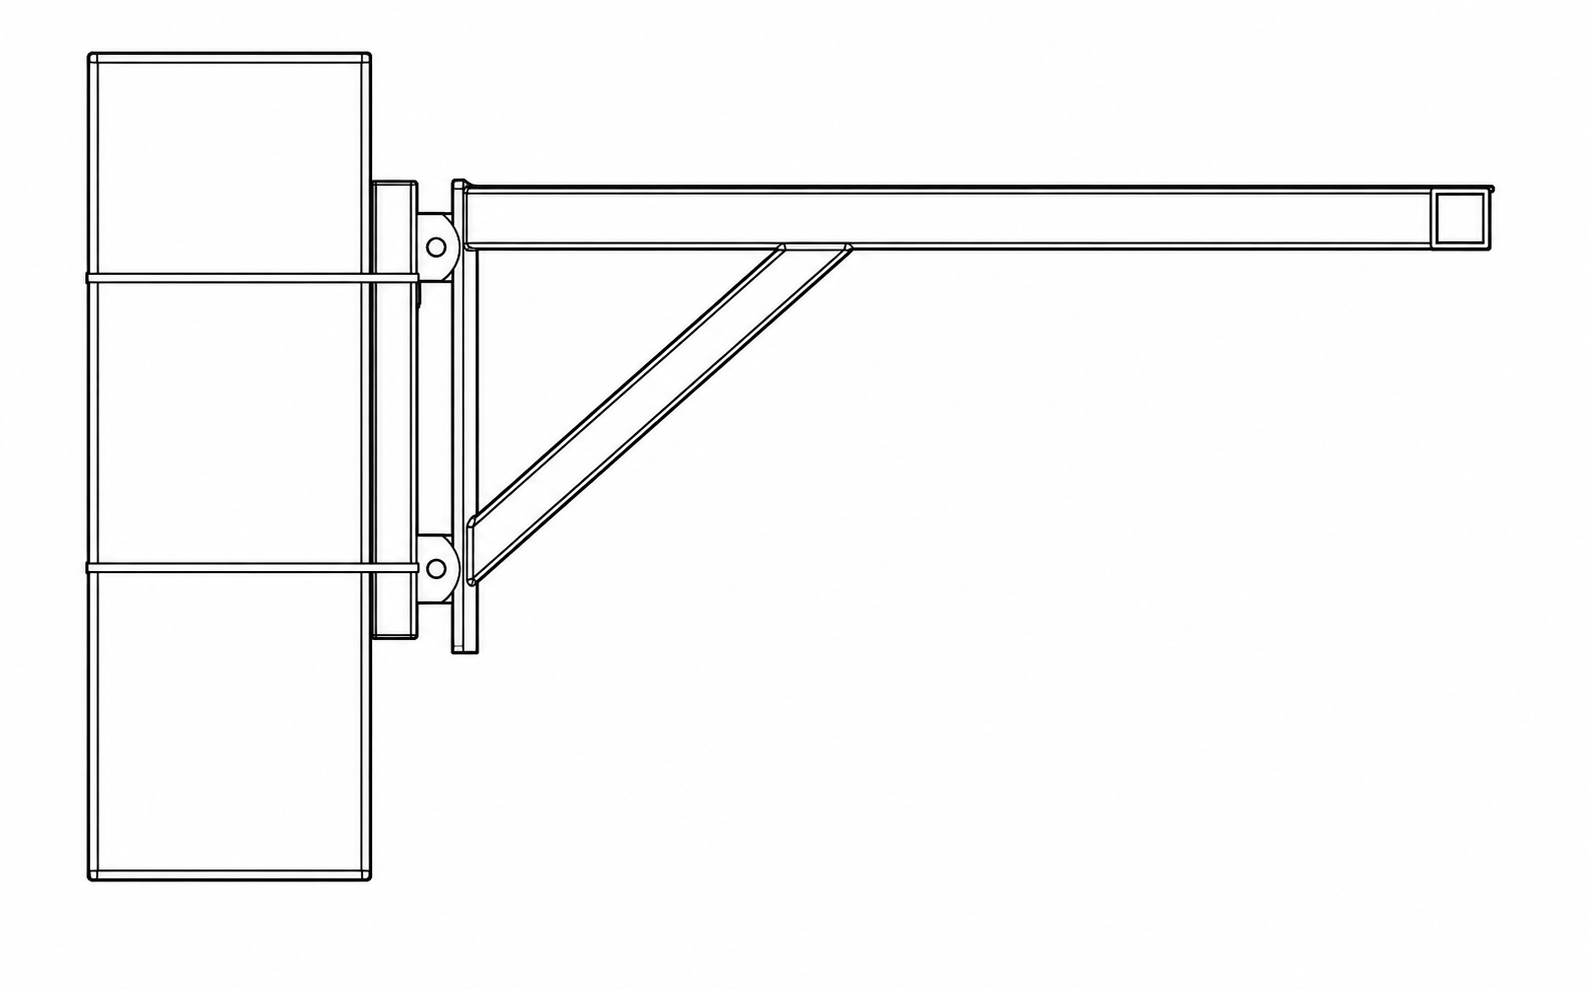
\includegraphics[width=\textwidth]{24_Halterung_Item_Kragarm.png}
        \caption{Item-Kragarm mit Strebe}
    \end{subfigure}
    \caption{Varianten der Kamerahalterung}
    \label{fig:hw-varianten}
\end{figure}

Gewählt wurde der Item-Kragarm. Das Profil wiegt mit \SI[per-mode=symbol]{0,93}{\kilo\gram\per\metre} nur etwa ein Drittel des Kantholzes (\SI[per-mode=symbol]{2,69}{\kilo\gram\per\metre}), und die Strebe entlastet die Verbindung zum Mast. Die Profile sind maßhaltig und lassen sich über ihre Nuten stufenlos verstellen. Der Arbeitsbereich bleibt frei. \Add{[OFFEN: weitere Gründe, z.\,B. Verfügbarkeit im Labor]}

Der Mast wird ohne Bohrung an der Säule gehalten. Zwei Ratschengurte im Abstand von \SI{300}{\milli\metre} umschlingen Säule und Mast und bilden ein Kräftepaar gegen das Kippmoment des Auslegers. Eine Gummimatte zwischen Mast und Säule erhöht die Reibung, ein Schlauchschellenband sichert zusätzlich. Zwei Gelenke verbinden Ausleger und Mast, sodass die Richtung des Auslegers einstellbar ist. Für diese Befestigung wurde eine Sicherheitsabschätzung erstellt. Sie betrachtet den Mast als starren Körper, den nur Gurtkraft und Reibung halten, und prüft drei Fälle:
\begin{itemize}
    \item \textbf{Klaffen.} Die obere Kontaktebene darf nicht abheben.
    \item \textbf{Rutschen.} Die Reibung muss das Gewicht tragen.
    \item \textbf{Torsion.} Steht der Ausleger schräg zur Säule, entsteht ein Moment um die Wandnormale, das nur die Reibung aufnehmen kann.
\end{itemize}
Maßgebend ist die Reibung aus Rutschen und Torsion zusammen. Ohne Sicherheitsfaktor ist eine Gurtkraft von \SI{65,8}{\newton} nötig. Bei einer geforderten Sicherheit von~3 ist die Befestigung zu \SI{56,5}{\percent} ausgelastet, die vorhandene Sicherheit beträgt \num{5,31}. Der Nachweis hält bis zu einem Reibwert von \num{0,36}, angenommen wurde \num{0,86} für Beton auf Stahl. Rechnung und Werte stehen in Anhang~\ref{app:Mechanik}.

Durch die Gelenke kann sich die Lage der Kamera ändern. Als Alternative zur Bestimmung der Kamerapose über die WorldTags wurde deshalb ein Drehgeber im Gelenk betrachtet (Abbildung~\ref{fig:hw-drehgeber}). Er misst den Winkel des Auslegers, aus dem ein Kinematikmodell mit einem Freiheitsgrad die Kamerapose berechnet. Ein Drehgeber kann nicht verdeckt werden, braucht aber zusätzliche Hardware, und das Spiel im Gelenk verfälscht die Messung. Mit den WorldTags muss die Halterung die Kamera nicht genau positionieren, sondern nur während einer Messung ruhig halten.

\begin{figure}[htbp]
    \centering
    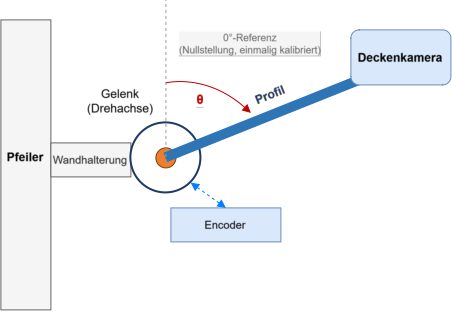
\includegraphics[width=0.5\textwidth]{25_WKS_Drehgeber.png}
    \caption{Verworfene Alternative zum Bezug auf das Weltkoordinatensystem: Drehgeber im Gelenk der Halterung}
    \label{fig:hw-drehgeber}
\end{figure}

Nach der ersten Montage zeigte sich, dass die Gurte die Drehung des Mastes um die Säule nicht halten. Nachgerüstet wurden zwei Querprofile, die an den Flächen der Säule anliegen (Abbildung~\ref{fig:hw-montage}). Sie stützen die Drehung formschlüssig ab und nicht mehr nur über Reibung. Die Abschätzung hatte die Torsion allein über Reibung mit dem vollen Reibwert betrachtet. \Add{[OFFEN: Ursache, z.\,B. Gummimatte, Vorspannung der Gurte, eckige Säule]} Am 12.10.2026 wurde die Halterung mit der Deckenkamera montiert.

\begin{figure}[htbp]
    \centering
    \begin{subfigure}[b]{0.24\textwidth}
        \centering
        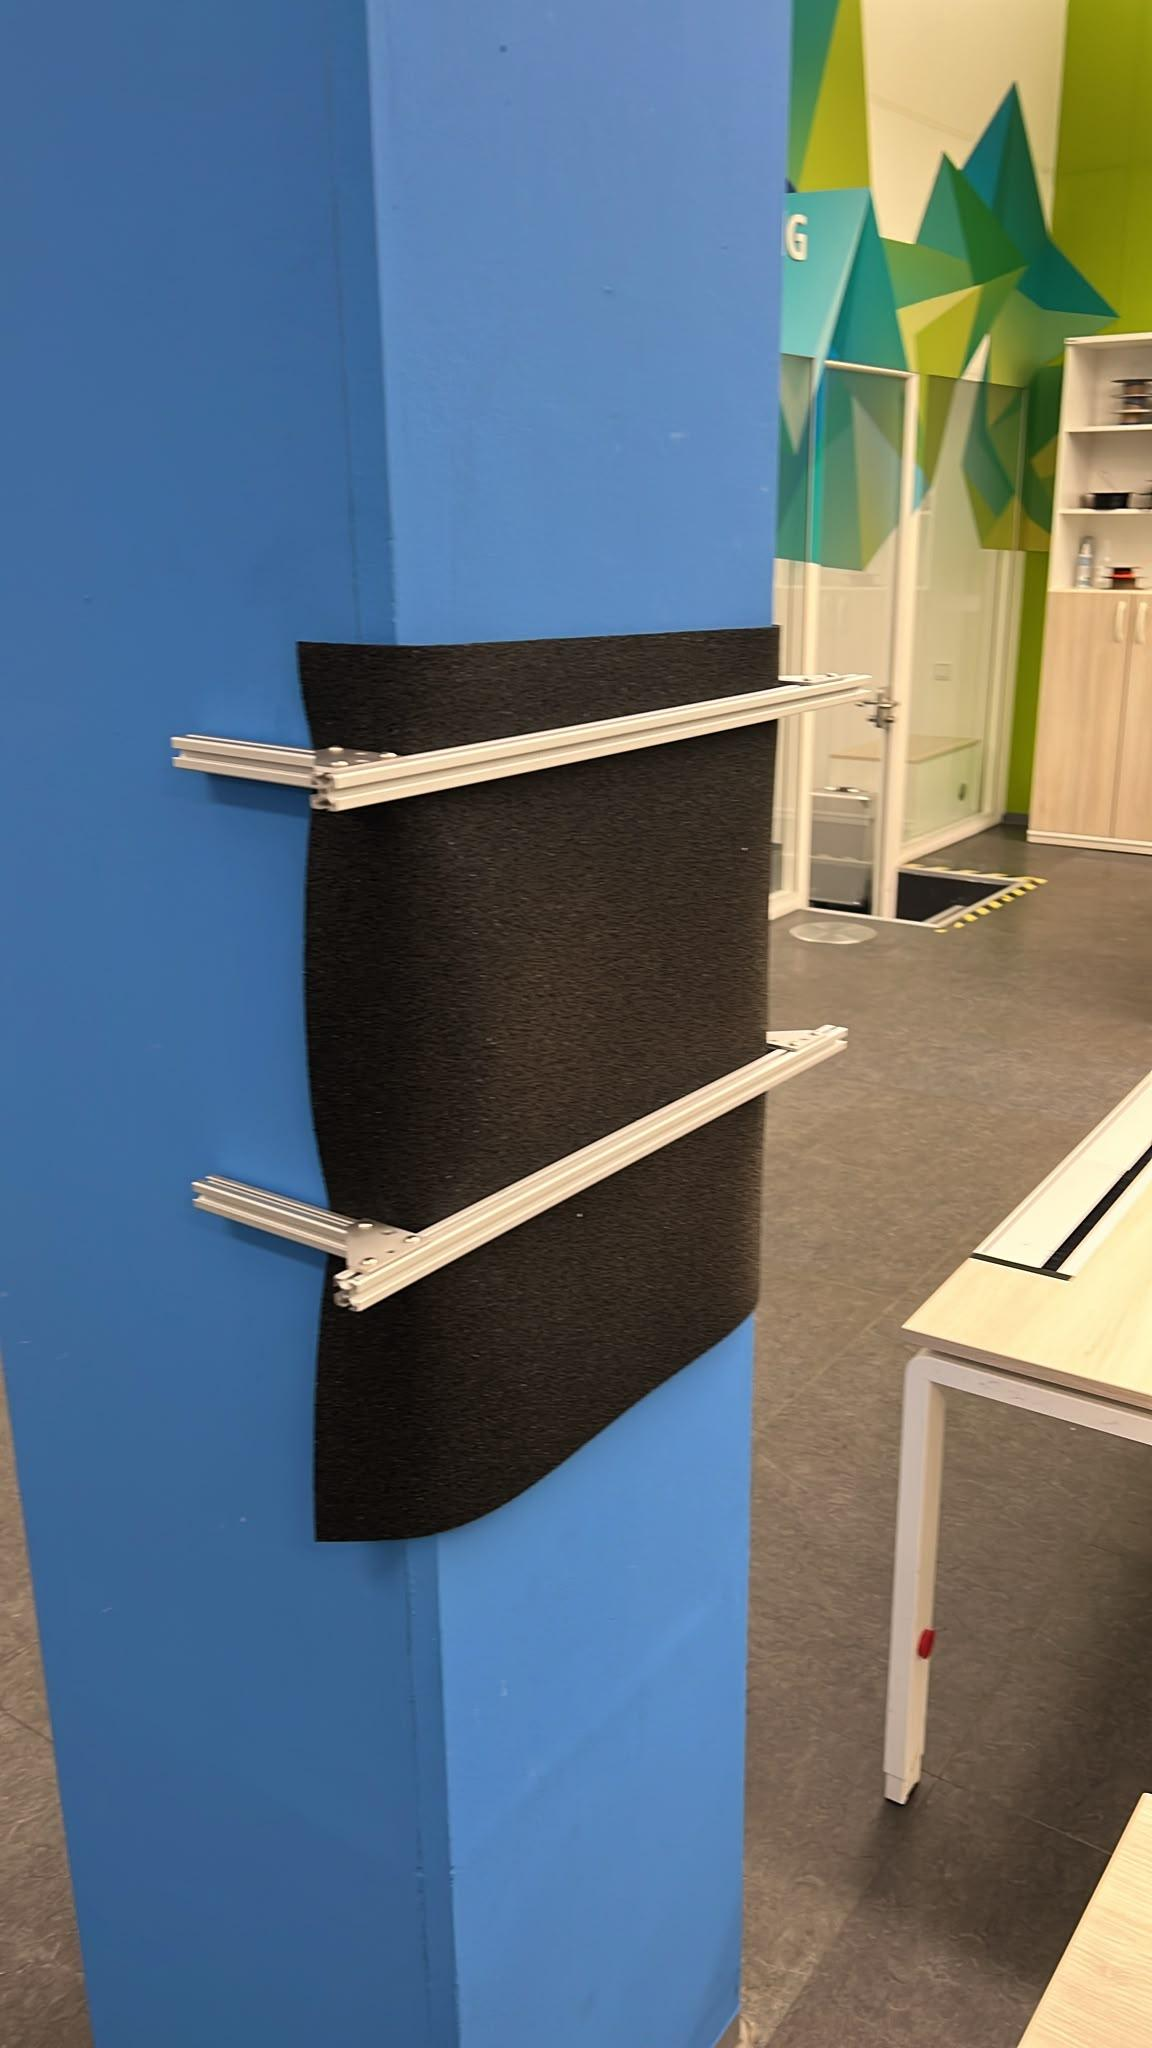
\includegraphics[width=\textwidth]{27_Halterung_Querprofil.jpg}
        \caption{Querprofile}
    \end{subfigure}\hfill
    \begin{subfigure}[b]{0.72\textwidth}
        \centering
        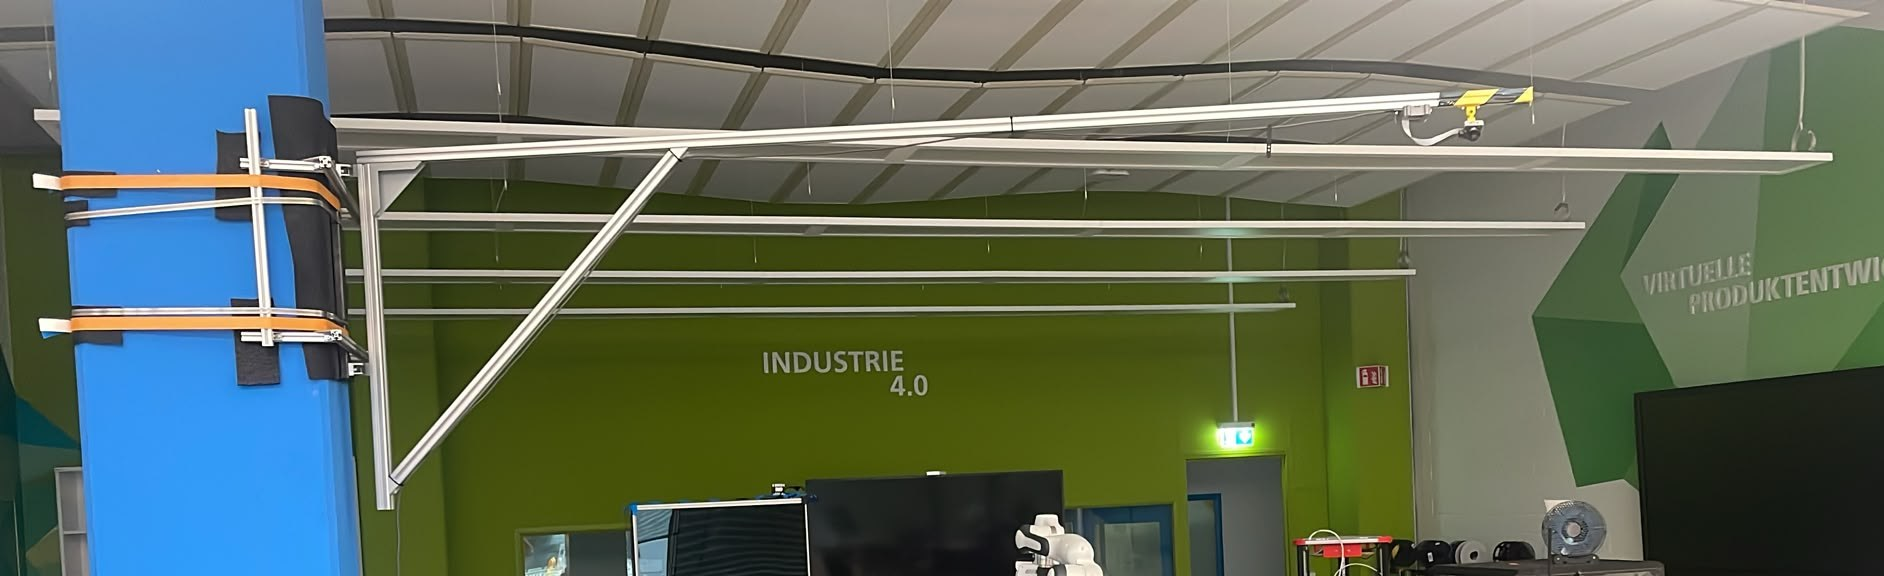
\includegraphics[width=\textwidth]{28_Halterung_montiert.jpg}
        \caption{Montierte Halterung mit Ausleger und Strebe}
    \end{subfigure}
    \caption{Kamerahalterung an der Säule}
    \label{fig:hw-montage}
\end{figure}

\subsection{AprilTags}
\label{subsec:hw-tags}
Verwendet werden AprilTags der Familie tag36h11. Die ModulTags haben eine Kantenlänge von \SI{80}{\milli\metre}, die vier WorldTags \SI{200}{\milli\metre}, jeweils gemessen am schwarzen Quadrat. Die Tags liegen flach auf ebenen Flächen, die ModulTags auf den Tischplatten und die WorldTags auf dem Boden. Ihre Lage lässt sich so von Bezugskanten aus messen. Die eingemessenen Lagen der WorldTags stehen in Anhang~\ref{app:Mechanik}.

Ein Tag muss eben sein und eine genaue Kantenlänge haben, sonst stimmen Abstand und Lage der geschätzten Pose nicht. Zunächst wurden die Tags auf Papier gedruckt. Danach wurden sie mit dem Laser auf Metall graviert (Abbildung~\ref{fig:hw-tag-gelasert}). Eine Mattlackierung veränderte die Oberfläche dieser Tags so stark, dass die Erkennung deutlich schlechter wurde. Eingesetzt werden deshalb laminierte Papiertags. \Add{[OFFEN: Gründe für die Wechsel; wie Kantenlänge und Ebenheit der laminierten Tags geprüft wurden]}

\begin{figure}[htbp]
    \centering
    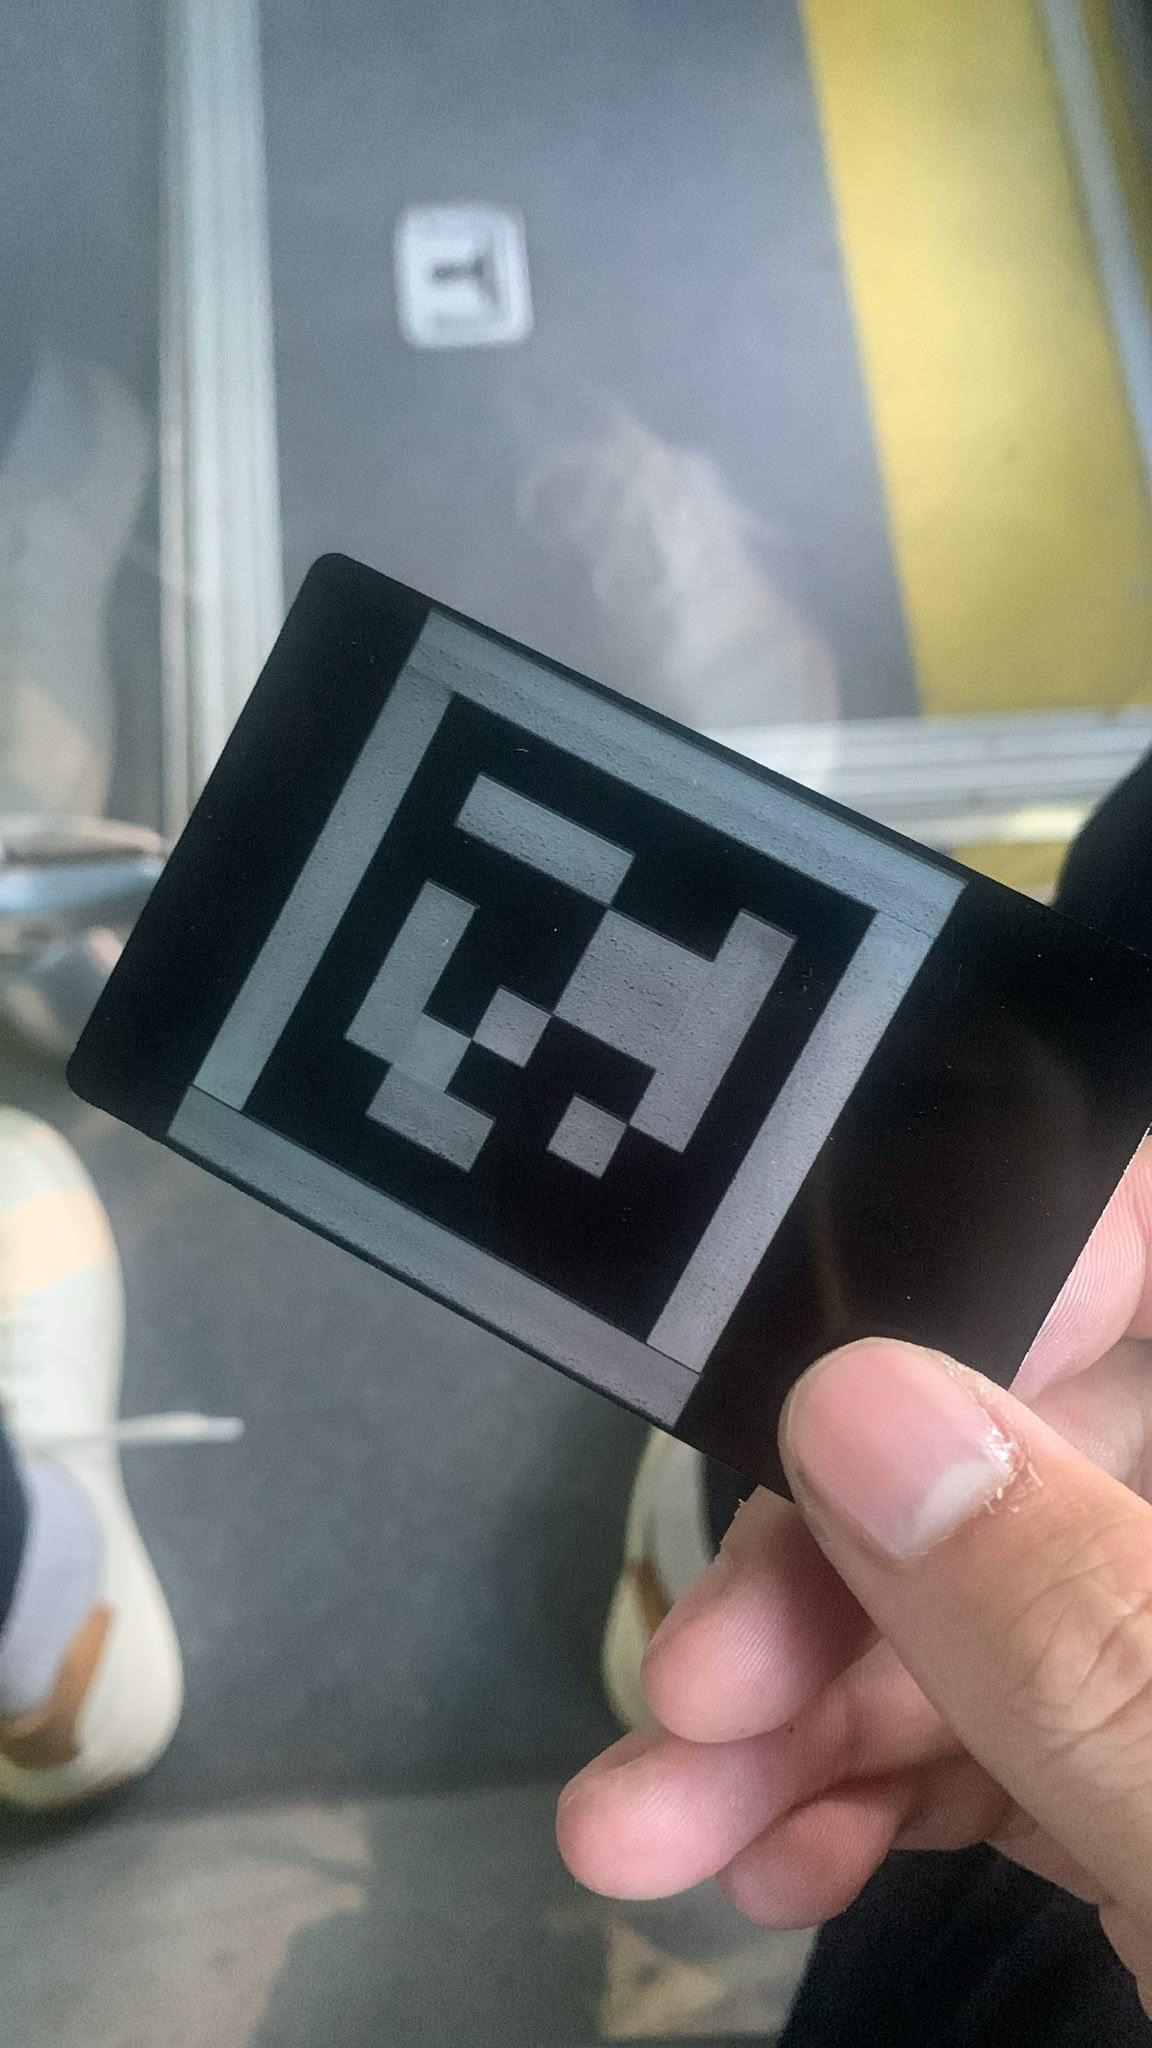
\includegraphics[width=0.2\textwidth]{26_Tag_gelasert.jpg}
    \caption{Lasergravierter AprilTag aus den Versuchen vom Juli 2026}
    \label{fig:hw-tag-gelasert}
\end{figure}


\section{Bildverarbeitung}
\label{sec:bildverarbeitung}
% Kommentare Meric und Sven (aus den Notizen übernommen): ICH GLAUBE DIE GANZE KALIBRIERUNG GEHÖRT SCHON HIER REIN UND SPÄTER IN DER VERIFKATION ZEIGEN WIR NUR WIE WIR DIE INTRINSIC VERIFIZIEREN? (Kommentar von Meric) JA ICH DENKE VOR ALLEM WEIL WIR JA AUCH AUTOMATISCH KALIBRIEREN UND EIN BESTAND TEIL DES KONZEPT IS PASST ES HIER GUT (Kommentar von Sven)
% -> Umgesetzt: Die Kalibrierung steht vollständig in diesem Abschnitt (Unterabschnitt Kalibrierung), die Ergebnisse in Kapitel Verifikation & Validierung.
Die Bildverarbeitung macht aus einem Kamerabild die Pose eines Moduls. Dafür muss sie die Abbildung der Kamera kennen, die Tags im Bild finden, ihre Pose schätzen und diese über eine Kette von Transformationen auf das Modul übertragen. Dieser Abschnitt beschreibt diese Schritte zunächst allgemein, danach die Kalibrierung der Kameras und schließlich die Umsetzung für Layer~1 und Layer~2.

\subsection{Kameramodell}
\label{subsec:bv-kameramodell}
Die Abbildung einer Kamera wird mit dem Lochkameramodell beschrieben. Ein Punkt $\mathbf{X} = (X, Y, Z)^{\mathsf{T}}$ im Raum wird auf den Bildpunkt $(u, v)$ projiziert:
\begin{equation}
    \lambda \begin{pmatrix} u \\ v \\ 1 \end{pmatrix}
    = \mathbf{K} \left[\, \mathbf{R} \mid \mathbf{t} \,\right] \begin{pmatrix} \mathbf{X} \\ 1 \end{pmatrix},
    \qquad
    \mathbf{K} = \begin{pmatrix} f_x & 0 & c_x \\ 0 & f_y & c_y \\ 0 & 0 & 1 \end{pmatrix}
    \label{eq:bv-lochkamera}
\end{equation}
Die Kameramatrix $\mathbf{K}$ enthält die Brennweiten $f_x$, $f_y$ in Pixeln und den Bildhauptpunkt $(c_x, c_y)$. Zusammen mit der Verzeichnung des Objektivs bildet sie die \emph{intrinsischen} Parameter. Diese hängen nur von Kamera und Objektiv ab. Rotation $\mathbf{R}$ und Translation $\mathbf{t}$ sind die \emph{extrinsischen} Parameter. Sie beschreiben die Lage der Kamera im Raum \cite{Hartley2004}.

Reale Objektive verzeichnen das Bild, sodass gerade Linien zum Bildrand hin gekrümmt erscheinen. Für Objektive mit kleinem Bildwinkel beschreibt das Modell nach Brown und Conrady die Verzeichnung mit drei radialen und zwei tangentialen Koeffizienten \cite{Brown1966}. Bei Weitwinkel- und Fischaugenobjektiven reicht dieses Modell nicht mehr aus. Das Modell nach Kannala und Brandt bildet stattdessen den Einfallswinkel $\theta$ eines Strahls über ein Polynom auf den Abstand vom Bildhauptpunkt ab \cite{Kannala2006}:
\begin{equation}
    \theta_d = \theta \left(1 + k_1 \theta^2 + k_2 \theta^4 + k_3 \theta^6 + k_4 \theta^8\right).
    \label{eq:bv-kannala}
\end{equation}
Die Deckenkamera mit ihrem Weitwinkelobjektiv wird deshalb nach Kannala und Brandt beschrieben, die Handkamera nach Brown und Conrady. Beide Modelle erwiesen sich in Bildtests am 29.09.2026 für die jeweilige Kamera als am besten geeignet. \Add{[OFFEN: Kennzahlen der Bildtests]}

\subsection{Erkennung der AprilTags}
\label{subsec:bv-erkennung}
Ein AprilTag besteht aus einem schwarzen Quadrat mit einem Raster aus hellen und dunklen Zellen. Bei der Familie tag36h11 sind es \numproduct{6 x 6} Zellen, die 36~Bit tragen. Zwei Codes der Familie unterscheiden sich in mindestens elf Bit. Dadurch lassen sich einzelne Lesefehler korrigieren, ohne dass ein Tag mit einem anderen verwechselt wird \cite{Olson2011,Wang2016}.

Die Erkennung läuft in mehreren Schritten ab \cite{GarridoJurado2014}:
\begin{enumerate}
    \item \textbf{Binarisieren.} Ein adaptiver Schwellwert trennt das Graubild in Schwarz und Weiß. Er vergleicht jedes Pixel mit seiner Umgebung und bleibt damit auch bei ungleichmäßiger Beleuchtung stabil.
    \item \textbf{Vierecke finden.} Im Binärbild werden Konturen gesucht und durch Polygone angenähert. Übrig bleiben konvexe Vierecke plausibler Größe.
    \item \textbf{Entzerren.} Jedes Viereck wird über eine projektive Transformation auf ein Quadrat abgebildet. Jede Zelle wird dabei mit mehreren Pixeln abgetastet, der unscharfe Zellrand bleibt unberücksichtigt.
    \item \textbf{Dekodieren.} Die gelesenen Bits werden in allen vier Drehlagen mit den Codes der Familie verglichen. Ein Tag gilt als erkannt, wenn höchstens so viele Bits abweichen, wie korrigiert werden dürfen. Die Drehlage legt fest, welche Ecke die erste ist.
    \item \textbf{Ecken bestimmen.} Die vier Ecken werden als Schnitt der Kanten bestimmt und können optional subpixelgenau verfeinert werden.
\end{enumerate}
Schwächen hat das Verfahren bei unscharfen oder kontrastarmen Bildern. Verwaschene Zellgrenzen führen zu falschen Bits, und kleine Tags haben zu wenige Pixel je Zelle. Eine höhere Fehlerkorrektur findet dann zwar mehr Tags, erhöht aber das Risiko falscher IDs.

\subsection{Posenschätzung}
\label{subsec:bv-pose}
Aus den vier Ecken und der bekannten Kantenlänge $s$ wird die Pose des Tags relativ zur Kamera geschätzt. Im Tag-Koordinatensystem liegen die Ecken bei $(\pm s/2, \pm s/2, 0)$. Gesucht sind $\mathbf{R}$ und $\mathbf{t}$, die diese Punkte nach Gleichung~\eqref{eq:bv-lochkamera} auf die gemessenen Bildpunkte abbilden. Diese Aufgabe heißt Perspective-n-Point-Problem (PnP). Für ein ebenes Quadrat löst sie das Verfahren IPPE geschlossen \cite{Collins2014}. Das Ergebnis ist die Transformation $\mathbf{T}_{\mathrm{Kamera,Tag}}$ mit sechs Freiheitsgraden, drei der Lage und drei der Orientierung.

Es handelt sich um eine Schätzung. Rauschen in den Bildpunkten der Ecken überträgt sich auf die Pose, und zwar am stärksten auf den Abstand entlang der Sichtlinie und auf die Neigung. Wie gut eine Pose zu den Messungen passt, zeigt der Reprojektionsfehler, also der mittlere Abstand zwischen den gemessenen Ecken $\mathbf{u}_i$ und den mit der geschätzten Pose projizierten Ecken $\hat{\mathbf{u}}_i$:
\begin{equation}
    e_{\mathrm{rep}} = \sqrt{\frac{1}{4} \sum_{i=1}^{4} \left\lVert \mathbf{u}_i - \hat{\mathbf{u}}_i \right\rVert^2 } .
    \label{eq:bv-reprojektion}
\end{equation}
Bei kleinen oder frontal gesehenen Tags liefert IPPE zwei fast gleich gute Lösungen, die sich in der Neigung des Tags unterscheiden. Ist der Fehler der besten Lösung größer als \SI{60}{\percent} des Fehlers der zweiten, gilt die Messung als \emph{mehrdeutig}. Ihre Position ist verwertbar, ihre Orientierung nicht. Um das Rauschen zu verringern, wird jede Pose über mehrere frische Bilder gemittelt, und Bilder mit zu großem Reprojektionsfehler werden verworfen.

\subsection{Transformationskette}
\label{subsec:bv-kette}
Aus der Pose eines Tags folgt die Pose seines Moduls:
\begin{equation}
    \mathbf{T}_{\mathrm{Welt,Modul}} = \mathbf{T}_{\mathrm{Welt,Kamera}} \cdot \mathbf{T}_{\mathrm{Kamera,Tag}} \cdot \mathbf{T}_{\mathrm{Tag,Modul}} .
    \label{eq:bv-kette}
\end{equation}
$\mathbf{T}_{\mathrm{Tag,Modul}}$ beschreibt, wo der Tag auf dem Modul sitzt, und stammt aus dem Modulkatalog (Abschnitt~\ref{sec:digitaler_zwilling}). Die beiden Ebenen unterscheiden sich nur darin, woher $\mathbf{T}_{\mathrm{Welt,Kamera}}$ kommt. Die Deckenkamera bestimmt ihre Pose aus den WorldTags im selben Bild. Für einen WorldTag $w$ mit eingemessener Lage gilt
\begin{equation}
    \mathbf{T}_{\mathrm{Welt,Kamera}} = \mathbf{T}_{\mathrm{Welt},w} \cdot \mathbf{T}_{\mathrm{Kamera},w}^{-1} .
    \label{eq:bv-kamerapose}
\end{equation}
Bei der Handkamera folgt die Kamerapose aus der Stellung des Roboters (Abschnitt~\ref{sec:servoing}). Algorithmus~\ref{alg:bv-layer1} fasst die Bildverarbeitung für Layer~1 zusammen.

\floatname{algorithm}{Algorithmus}
\renewcommand{\algorithmicrequire}{\textbf{Eingabe:}}
\renewcommand{\algorithmicensure}{\textbf{Ausgabe:}}
\begin{algorithm}[htbp]
    \caption{Lokalisierung der Module mit der Deckenkamera (Layer~1)}
    \label{alg:bv-layer1}
    \begin{algorithmic}[1]
        \Require Kalibrierung $\mathbf{K}$, Verzeichnung; Modulkatalog mit WorldTags und ModulTags
        \Ensure grobe Pose $\mathbf{T}_{\mathrm{Welt,Modul}}$ jedes erkannten Moduls
        \For{jedes von drei frischen Bildern}
            \State Tags erkennen: binarisieren, Vierecke finden, entzerren, dekodieren
            \ForAll{erkannten Tags}
                \State $\mathbf{T}_{\mathrm{Kamera,Tag}}$ mit IPPE schätzen
                \State verwerfen, wenn $e_{\mathrm{rep}}$ zu groß
            \EndFor
            \State $\mathbf{T}_{\mathrm{Welt,Kamera}}$ aus den WorldTags nach Gl.~\eqref{eq:bv-kamerapose}
            \ForAll{ModulTags}
                \State Lage: Sehstrahl zur Tag-Mitte mit der Tag-Höhe aus dem Katalog schneiden
                \State Orientierung: nur die Drehung um die Hochachse übernehmen
            \EndFor
        \EndFor
        \State Lage und Drehung jedes Tags über die Bilder mitteln
        \ForAll{Module}
            \State $\mathbf{T}_{\mathrm{Welt,Modul}}$ nach Gl.~\eqref{eq:bv-kette}, gemittelt über alle Tags des Moduls
        \EndFor
    \end{algorithmic}
\end{algorithm}

\subsection{Kalibrierung}
\label{subsec:bv-kalibrierung}
Für eine Messung müssen drei Größen bekannt sein: die intrinsischen Parameter beider Kameras, die Lage der Handkamera am Flansch und die Lage der WorldTags. Die WorldTags werden einmal eingemessen (Anhang~\ref{app:Mechanik}). Die beiden anderen Größen bestimmt das System selbst mithilfe des Roboters, ohne dass eine Kamera abgebaut werden muss. Fehlt beim Start eine Kalibrierung oder passt sie nicht zur eingestellten Auflösung, wird sie neu erstellt (Abschnitt~\ref{sec:gesamtarchitektur}).

\paragraph{Intrinsische Kalibrierung.}
Die Kamera nimmt ein Schachbrett bekannter Feldgröße aus vielen Lagen auf. Aus den erkannten Ecken werden Kameramatrix und Verzeichnung so geschätzt, dass die Ecken möglichst genau auf ihre gemessenen Bildpunkte fallen \cite{Zhang2000}. Verwendet wird ein Schachbrett mit \numproduct{7 x 10} Innenecken und \SI{23}{\milli\metre} Feldgröße. Die ungerade Summe der Eckenzahlen macht die Lage des Bretts eindeutig, sodass eine Drehung um \SI{180}{\degree} erkannt wird. Die Aufnahmen übernimmt der Roboter. Für die Deckenkamera hält er das Brett an 16~Positionen, die der Bediener einmal einlernt. Werden mehr Bilder als Positionen gebraucht, fährt er die Positionen erneut ab und dreht dabei das Handgelenk jeweils etwas anders, sodass das Brett unter einem anderen Winkel erscheint. Für die Handkamera ist das Brett vor dem Roboter befestigt, und der Roboter fährt die Kamera um das Brett.

\paragraph{Hand-Auge-Kalibrierung.}
Die Lage der Handkamera am Flansch, $\mathbf{X} = \mathbf{T}_{\mathrm{Flansch,Kamera}}$, ist konstant, aber unbekannt. Zu ihrer Bestimmung sieht die Handkamera ein fest stehendes Kalibrierbrett aus vielen Roboterposen. In jeder Pose $i$ ist die Lage des Flansches $\mathbf{T}_{\mathrm{Basis,Flansch},i}$ aus den Gelenkwinkeln bekannt, die Lage des Bretts $\mathbf{T}_{\mathrm{Kamera,Brett},i}$ wird gemessen. Weil das Brett stillsteht, gilt für je zwei Posen $i$ und $j$
\begin{equation}
    \mathbf{A}\mathbf{X} = \mathbf{X}\mathbf{B}
    \quad\text{mit}\quad
    \mathbf{A} = \mathbf{T}_{\mathrm{Basis,Flansch},j}^{-1}\, \mathbf{T}_{\mathrm{Basis,Flansch},i},
    \quad
    \mathbf{B} = \mathbf{T}_{\mathrm{Kamera,Brett},j}\, \mathbf{T}_{\mathrm{Kamera,Brett},i}^{-1} .
    \label{eq:bv-axxb}
\end{equation}
$\mathbf{A}$ ist die Bewegung des Flansches zwischen beiden Posen, $\mathbf{B}$ die dabei gemessene Bewegung der Kamera. Eine geschlossene Lösung liefert das Verfahren nach Park und Martin \cite{ParkMartin1994}. Sie dient als Startwert für eine Verfeinerung, die $\mathbf{X}$ und die Lage des Bretts gemeinsam so anpasst, dass der Reprojektionsfehler aller Brettecken minimal wird. Die Verfeinerung gewichtet große Fehler nach Huber schwächer, und Aufnahmen mit auffällig großem Fehler werden verworfen. Optional wird ein Maßstab mitgeschätzt, der Fehler in der Feldgröße oder in der Intrinsik auffängt. Als Gütemaß dient der Vorhersagefehler, wenn jeweils eine Aufnahme ausgelassen und aus den übrigen vorhergesagt wird.

Genau wird die Lösung nur, wenn die Drehungen zwischen den Posen groß sind und um Achsen in alle Richtungen erfolgen \cite{Tsai1989}. Liegen zudem alle Aufnahmen im selben Abstand, lässt sich der Abstand der Linse vom Flansch kaum vom Maßstab des Bretts unterscheiden. Der digitale Zwilling plant die Aufnahmeposen deshalb selbst in drei Gruppen. Die erste blickt senkrecht auf das Brett, um die Sichtlinie um bis zu \SI{90}{\degree} gedreht und aus zwei Abständen. Die zweite ist ein Ring mit \SI{25}{\degree} Neigung, alle \SI{60}{\degree} um das Brett. Die dritte ist ein Ring mit \SI{40}{\degree} Neigung im 1,3-fachen Abstand, versetzt dazwischen. Die Drehungen um die Sichtlinie wechseln dabei ihr Vorzeichen. Jeder Ring wird einmal umrundet, damit der Roboter nicht hin und her fährt, und unerreichbare Posen entfallen. Nach jeder Aufnahme liest der Zwilling die Gelenkwinkel erneut. Hat sich der Arm währenddessen bewegt, wird die Aufnahme wiederholt.

\paragraph{9-Punkte-Prüfung.}
Ein fester Versatz, der alle Aufnahmen gleich verschiebt, ist in der Streuung der Kalibrierung nicht zu sehen. Deshalb wird $\mathbf{X}$ zusätzlich mit dem Werkzeug des Roboters geprüft. Auf dem Tisch liegt ein Blatt mit vier ArUco-Markern und neun Kreuzen im Abstand von \SI{30}{\milli\metre}. Die Handkamera vermisst das Blatt. Die Lage jedes Kreuzes folgt dabei aus dem Sehstrahl durch das Kreuz, geschnitten mit der Tischebene, weil die Tischhöhe genauer bekannt ist als der Abstand aus der Kamera. Danach fährt der Roboter einen im Greifer gehaltenen Stift nacheinander über jedes Kreuz. Zwischen zwei Kreuzen hebt er ihn an, sodass der Stift nie über das Blatt schleift. Der Bediener trägt ein, wie weit die Stiftspitze neben dem Kreuz steht. Aus den neun Versätzen werden Verschiebung, Drehung und Maßstab geschätzt und als Korrektur in $\mathbf{X}$ übernommen. Eine Drehung entspricht dabei einer Drehung der Kamera um ihre Blickachse, ein Maßstab einem Fehler in der Kamerahöhe. Korrekturen über \SI{2}{\centi\metre} oder \SI{2}{\degree} lehnt der Hand-Pi ab, weil sie auf einen Fehler bei der Eingabe hindeuten. Wie gut die Kalibrierung ist und wie lange sie dauert, zeigt Kapitel~\ref{ch:Verifikation}.

\subsection{Umsetzung für Layer~1}
\label{subsec:bv-layer1}
Abbildung~\ref{fig:bv-layer1} zeigt den Ablauf eines Layer-1-Scans. Die Deckenkamera nimmt mit voller Sensorauflösung von \numproduct{4056 x 3040} Pixeln bei höchstens zehn Bildern je Sekunde auf. In halber Auflösung würden die ModulTags aus der Deckenhöhe zu klein abgebildet.

\begin{figure}[htbp]
    \centering
    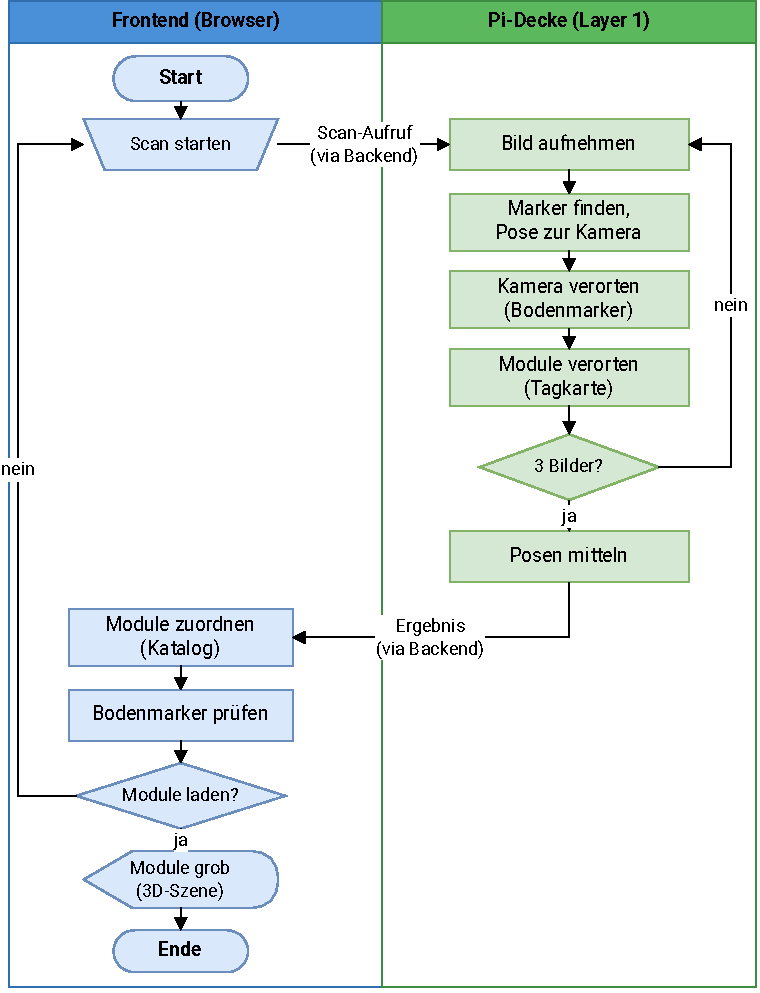
\includegraphics[width=0.6\textwidth]{04_Layer1_Scan_v3.pdf}
    \caption{Ablauf des Layer-1-Scans}
    \label{fig:bv-layer1}
\end{figure}

Bei der Inbetriebnahme fand der Detektor nicht alle Tags. Die Kanten im Bild waren \SIrange{4}{8}{Pixel} breit, bei nur \SIrange{6}{13}{Pixel} je Zelle. Weil die Unschärfe keine Vorzugsrichtung hatte, schied Bewegungsunschärfe aus. Die Ursache war ein Fokusfehler. Nach dem Nachstellen des Fokus findet der Detektor mit den Standardeinstellungen von OpenCV alle Tags. Zusätzlich wird jede Zelle beim Entzerren mit acht statt vier Pixeln abgetastet. Das gibt Reserve bei schlechterem Bild, ohne Fehlerkennungen zu erzeugen. Verworfen wurden drei Alternativen:
\begin{itemize}
    \item \textbf{Höhere Fehlerkorrektur.} Sie findet mehr Tags, liefert bei Bildrauschen aber falsche IDs. Für die Zellüberwachung, die auf fehlende und neue Tags reagiert, ist das der falsche Tausch.
    \item \textbf{Kontrastverstärkung (CLAHE).} Sie erzeugt aus verstärktem Rauschen Tags, die es nicht gibt.
    \item \textbf{Subpixelgenaue Eckenverfeinerung.} Das Verfahren aus AprilTag ist etwa zwanzigmal langsamer und verliert Tags. Das einfachere Verfahren verschiebt die Ecken nur um \numrange{0,1}{0,3}~Pixel.
\end{itemize}

Der Abstand eines Tags aus seiner Bildgröße streut bei mehreren Metern Entfernung um Zentimeter. Bei schrägem Blick wird dieser Tiefenfehler zu einem Fehler in der Ebene, bei \SI{45}{\degree} etwa im Verhältnis 1:1. Weil die Module auf dem Boden stehen, ist die Höhe jedes Tags aus dem Katalog bekannt. Die Lage wird deshalb als Schnitt des Sehstrahls von der Kamera zur Tag-Mitte mit dieser Höhe bestimmt, und der geschätzte Abstand fließt nicht ein. Aus der Orientierung wird nur die Drehung um die Hochachse übernommen. Die Neigung eines kleinen Tags aus Metern Entfernung ist Rauschen und würde über den Hebel zum Modulursprung große Fehler erzeugen. Gemittelt wird über drei Bilder, Bilder mit einem Reprojektionsfehler über \SI{3}{Pixel} werden verworfen.

\subsection{Zellüberwachung auf dem Decken-Pi}
\label{subsec:bv-zellueberwachung}
Die Zellüberwachung aus Abschnitt~\ref{sec:gesamtarchitektur} läuft auf dem Decken-Pi. Etwa alle zwei Sekunden vergleicht er die erkannten Tags mit einer Referenz, dem zuletzt übernommenen Layer-1-Scan. Er unterscheidet drei Änderungen: Ein Modul wurde verschoben, ist hinzugekommen oder ist verschwunden. Als verschoben gilt ein Modul ab einer Abweichung von \SI{5}{\centi\metre} oder \SI{10}{\degree}. Gemeldet wird eine Änderung erst, wenn sie mindestens \SI{5}{\second} ohne Unterbrechung besteht, sodass eine einzelne Fehlmessung keinen Alarm auslöst. \Add{[OFFEN: Schwelle mit Abschnitt~\ref{sec:gesamtarchitektur} und Abbildung~\ref{fig:dz-ergebnis} abgleichen, dort \SI{15}{\centi\metre}]}

Für die Drehung genügt der Kurs eines Moduls. Liegt ein Tag flach, unterscheiden sich die beiden Lösungen einer mehrdeutigen Pose (Abschnitt~\ref{subsec:bv-pose}) nur in der Neigung, sodass ihr Kurs trotzdem verlässlich ist. In einer Simulation mit Draufsicht aus \SI{2,5}{\metre} waren 225 von 300 Posen mehrdeutig, der Kursfehler beider Lösungen betrug dabei höchstens \SI{6}{\degree}.

Schwieriger ist die Frage, wann ein Tag verschwunden ist. Nicht jeder Tag wird in jedem Bild erkannt. Am Decken-Pi wurde für einzelne Tags eine Erkennungsrate von nur \SI{40}{\percent} gemessen. Würde die Überwachung eine feste Zahl von Fehlbildern abwarten, meldete sie solche Tags laufend als verschwunden. Die Zahl $n$ der geforderten Fehlbilder hängt deshalb von der Erkennungsrate $r$ des Tags ab. Sie wird so gewählt, dass ein vorhandener Tag die Bilder nur mit einer Wahrscheinlichkeit unter $10^{-5}$ zufällig hintereinander verpasst:
\begin{equation}
    (1 - r)^n < 10^{-5}
    \quad\Rightarrow\quad
    n = \left\lceil \frac{\ln 10^{-5}}{\ln(1 - r)} \right\rceil, \qquad 3 \le n \le 60 .
    \label{eq:bv-fehlbilder}
\end{equation}
Die obere Grenze sorgt dafür, dass auch ein schlecht erkannter Tag nach spätestens zwei Minuten als fehlend gemeldet wird. Weil die Rate aus wenigen Bildern geschätzt wird und stark streut, geht die untere Grenze ihres 95-\%-Konfidenzintervalls nach Wilson ein \cite{Wilson1927}. Eine zu hoch geschätzte Rate würde zu wenige Fehlbilder fordern. In einer Simulation ergab eine Schranke von $10^{-4}$ noch einen Fehlalarm in zehn Stunden, mit $10^{-5}$ gab es in 20~Stunden keinen. Tags mit einer Erkennungsrate unter \SI{50}{\percent} werden als unsicher erkannt gekennzeichnet.

Die Überwachung lässt sich pausieren. Nennt der Aufrufer keine Dauer, endet die Pause nach zehn Minuten, spätestens aber nach einer Stunde, auch wenn niemand sie aufhebt. So läuft die Überwachung selbst dann weiter, wenn das Frontend abstürzt.

\subsection{Umsetzung für Layer~2}
\label{subsec:bv-layer2}
Die Handkamera misst Tags aus der Nähe. Jede Abweichung der Ecken wirkt dort als fester Versatz der Pose. Deshalb ist die subpixelgenaue Eckenverfeinerung hier eingeschaltet, die Rechenzeit spielt bei \numproduct{640 x 480} Pixeln keine Rolle. Bilder mit einem Reprojektionsfehler über \SI{1,5}{Pixel} werden verworfen.

Gemessen wird nur auf Abruf über die Methode \texttt{MeasureTags}. Sie wertet ausschließlich Bilder aus, die nach dem Aufruf eintreffen, also nie ein Bild aus der Fahrt. Je Tag liefert sie die über drei Bilder gemittelte Pose $\mathbf{T}_{\mathrm{Kamera,Tag}}$, die Angabe, ob die Messung mehrdeutig ist, die Zahl der Bilder mit dem Tag, den Reprojektionsfehler und die Bildränder, denen der Tag nahekommt. Mit diesen Angaben führt die Steuerung die Kamera nach (Abschnitt~\ref{sec:servoing}).

\begin{figure}[htbp]
    \centering
    \fbox{\parbox[c][4cm][c]{0.8\textwidth}{\centering\Add{[BILD OFFEN: Bild der Handkamera mit erkanntem Tag und eingeblendetem Achsenkreuz]}}}
    \caption{Bild der Handkamera mit erkanntem Tag und eingeblendetem Koordinatensystem}
    \label{fig:bv-tagbild}
\end{figure}


\section{Visual Servoing}
\label{sec:servoing}
Beim Visual Servoing wird die Bewegung eines Roboters über Informationen aus Kamerabildern geregelt \cite{Hutchinson1996}. Hier dient es dazu, die Handkamera an jeden Tag heranzuführen. Layer~1 kennt die Lage der Module nur auf einige Zentimeter genau. Fährt der Roboter allein nach dieser Lage vor einen Tag, liegt der Tag im nahen Bild schief, am Rand oder gar nicht im Bild. Die Kamera wird deshalb so lange nachgeführt, bis sie den Tag mittig und aus einem festen Abstand sieht. Das hat zwei Gründe. Erstens ist die Kalibrierung in der Bildmitte am genauesten, weil die Verzeichnung zum Rand hin zunimmt. Zweitens wurden Intrinsik und Hand-Auge-Kalibrierung der Handkamera weitgehend für einen festen Arbeitsabstand optimiert.

\subsection{Grundlagen}
\label{subsec:vs-grundlagen}
Beim Visual Servoing gibt es zwei Grundformen \cite{Chaumette2006}. Das bildbasierte Verfahren (IBVS) regelt direkt auf Merkmale im Bild, etwa die Ecken eines Tags. Das positionsbasierte Verfahren (PBVS) schätzt aus dem Bild zuerst eine Pose und regelt auf diese. Gewählt wurde PBVS, weil die Pose des Tags ohnehin vorliegt (Abschnitt~\ref{subsec:bv-pose}) und das Ziel einer Messung eine Pose ist und kein Bild.

Jede Messung wird über die Stellung des Roboters in sein Basiskoordinatensystem übertragen:
\begin{equation}
    \mathbf{T}_{\mathrm{Basis,Tag}} = \mathbf{T}_{\mathrm{Basis,Flansch}}(\mathbf{q}) \cdot \mathbf{T}_{\mathrm{Flansch,Kamera}} \cdot \mathbf{T}_{\mathrm{Kamera,Tag}} .
    \label{eq:vs-kette}
\end{equation}
$\mathbf{T}_{\mathrm{Basis,Flansch}}(\mathbf{q})$ folgt aus der Vorwärtskinematik der gelesenen Gelenkwinkel $\mathbf{q}$, und $\mathbf{T}_{\mathrm{Kamera,Tag}}$ ist die Messung der Handkamera. Die Hand-Auge-Transformation $\mathbf{X} = \mathbf{T}_{\mathrm{Flansch,Kamera}}$ stammt aus der Kalibrierung (Abschnitt~\ref{subsec:bv-kalibrierung}).

\subsection{Regelung im Stop-and-go}
\label{subsec:vs-regelung}
Der Roboter fährt im Wechsel: Er fährt, steht still, misst und korrigiert. Eine kontinuierliche Regelung scheidet aus zwei Gründen aus. Die Schnittstelle des Roboters nimmt Zielwerte für die Gelenkwinkel an, aber keine Geschwindigkeiten. Und ein Bild aus der Fahrt passt nicht sicher zu den gleichzeitig gelesenen Gelenkwinkeln, sodass schon wenige Millisekunden Versatz die Messung um Millimeter verschieben. Stop-and-go ist langsamer, doch für die Lokalisierung zählt die Genauigkeit und nicht die Taktzeit (A4).

Nach jedem Fahrbefehl gilt der Roboter erst als angekommen, wenn sich seine Gelenke in drei aufeinanderfolgenden Abfragen um weniger als \SI{0,0005}{\radian} bewegen. Erst dann wird gemessen. $\mathbf{T}_{\mathrm{Basis,Flansch}}(\mathbf{q})$ wird aus den dann gelesenen Gelenkwinkeln berechnet und nicht aus dem Fahrziel. Eine Abweichung zwischen Ziel und erreichter Stellung geht so nicht in die Messung ein.

Aus der gemessenen Tag-Mitte $\mathbf{p}_{\mathrm{Tag}}$, der Blickrichtung $\mathbf{a}$ der Kamera und dem Sollabstand $s$ ergibt sich das Ziel der Kamera:
\begin{equation}
    \mathbf{p}^{*}_{\mathrm{Kamera}} = \mathbf{p}_{\mathrm{Tag}} - s \cdot \mathbf{a} .
    \label{eq:vs-ziel}
\end{equation}
Die Kamera behält dabei ihre Blickrichtung und wird nur verschoben. Je Schritt fährt sie höchstens \SI{5}{\centi\metre}, damit eine Fehlmessung den Arm nicht weit schicken kann. Als zentriert gilt der Tag bei einer seitlichen Abweichung unter \SI{5}{\milli\metre} und einer Abstandsabweichung unter \SI{10}{\milli\metre}. Ein Schritt wird nur ausgeführt, wenn der Tag in mindestens zwei Bildern gefunden wurde. Ist der Tag nicht oder nur am Bildrand zu sehen, schwenkt die Kamera in Richtung des gemeldeten Bildrands. Fehlt er ganz, fährt sie eine Folge von Blickrichtungen ab. Abbildung~\ref{fig:vs-zentrieren} zeigt diesen Regelkreis.

\begin{figure}[htbp]
    \centering
    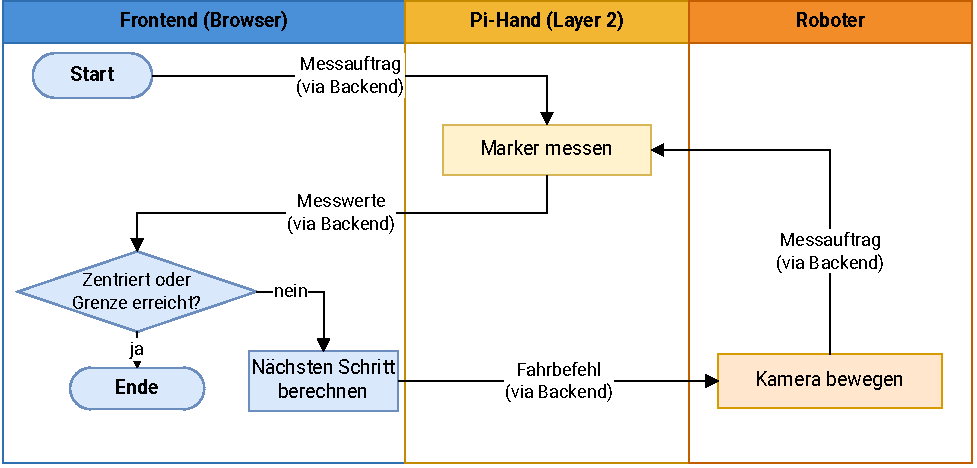
\includegraphics[width=0.85\textwidth]{05b_Zentrieren_v3.pdf}
    \caption{Regelkreis beim Zentrieren eines Tags}
    \label{fig:vs-zentrieren}
\end{figure}

Ist der Tag zentriert, fährt die Kamera entlang der Sichtlinie näher heran. Je näher sie ist, desto mehr Pixel hat der Tag und desto genauer wird die Pose. Der Nahabstand ist erreicht, wenn das schwarze Quadrat mit der Kantenlänge $t$ einen Anteil $k$ der kurzen Bildseite füllt. Bei einem halben Bildwinkel $\varphi$ gilt
\begin{equation}
    d_{\mathrm{nah}} = \frac{t/2}{k \cdot \tan\varphi} .
    \label{eq:vs-nahabstand}
\end{equation}
Mit $\varphi = \SI{21}{\degree}$, $k = \num{0,75}$ und $t = \SI{80}{\milli\metre}$ liegt der Nahabstand bei etwa \SI{14}{\centi\metre}. Vorrang haben ein Mindestabstand von \SI{12}{\centi\metre} und ein Abstand von \SI{5}{\centi\metre} zwischen Werkzeugspitze und Tag-Ebene.

Aus der Nahposition wird der Tag zusätzlich aus Ansichten gemessen, die um etwa \SI{12}{\degree} um seine Achsen gekippt sind. Ist eine Ansicht nicht erreichbar, kommen Ersatzansichten mit bis zu \SI{24}{\degree} hinzu. Ein fester Messfehler einer einzelnen Blickrichtung mittelt sich so teilweise heraus, und die Drehung des Tags wird erst durch übereinstimmende Ansichten belastbar. Die Messungen werden wie folgt vereint:
\begin{itemize}
    \item \textbf{Lage und Orientierung.} Die Lage ist das Mittel aller Ansichten, die Orientierung das Mittel der eindeutigen Ansichten.
    \item \textbf{Ausreißer.} Ab drei Messungen wird höchstens eine verworfen. Sie muss mehr als \SI{3}{\milli\metre} bzw. \SI{1}{\degree} vom Mittel der übrigen abweichen, und die übrigen müssen untereinander auf \SI{1,5}{\milli\metre} bzw. \SI{0,5}{\degree} übereinstimmen.
    \item \textbf{Mindestzahl.} Eine Modulpose wird nur aus mindestens drei Messungen gebildet.
    \item \textbf{Drehung.} Die Drehung des Moduls wird nur übernommen, wenn mindestens zwei eindeutige Ansichten auf \SI{0,5}{\degree} übereinstimmen. Andernfalls bleibt die Drehung aus Layer~1 erhalten, und der Vorschlag weist darauf hin.
\end{itemize}
Algorithmus~\ref{alg:vs-tag} fasst die Messung eines Tags zusammen.

\begin{algorithm}[htbp]
    \caption{Zentrieren und Messen eines Tags (Layer~2)}
    \label{alg:vs-tag}
    \begin{algorithmic}[1]
        \Require grobe Pose $\hat{\mathbf{T}}_{\mathrm{Basis,Tag}}$ aus Layer~1, Sollabstand $s$
        \Ensure gemessene Pose $\mathbf{T}_{\mathrm{Basis,Tag}}$ oder Abbruch
        \State Kamerapose $s$ vor dem Tag planen, prüfen und anfahren
        \Repeat
            \State Stillstand abwarten, Gelenkwinkel $\mathbf{q}$ lesen
            \State $\mathbf{T}_{\mathrm{Kamera,Tag}} \gets$ \texttt{MeasureTags} (nur frische Bilder)
            \If{Tag nicht oder am Rand gefunden}
                \State in Richtung des Bildrands schwenken bzw. Suchfolge fortsetzen
            \Else
                \State $\mathbf{T}_{\mathrm{Basis,Tag}} \gets \mathbf{T}_{\mathrm{Basis,Flansch}}(\mathbf{q})\,\mathbf{X}\,\mathbf{T}_{\mathrm{Kamera,Tag}}$
                \State Ziel $\mathbf{p}^{*}_{\mathrm{Kamera}}$ nach Gl.~\eqref{eq:vs-ziel}, Schritt auf \SI{5}{\centi\metre} begrenzen
                \State Schritt auf Erreichbarkeit und Kollision prüfen und fahren
            \EndIf
        \Until{zentriert oder Höchstzahl an Schritten erreicht}
        \State auf $d_{\mathrm{nah}}$ nach Gl.~\eqref{eq:vs-nahabstand} heranfahren und messen
        \ForAll{gekippten Ansichten}
            \If{erreichbar und kollisionsfrei} \State anfahren und messen \EndIf
        \EndFor
        \State Messungen vereinen, Ausreißer verwerfen, Mindestzahl und Drehung prüfen
    \end{algorithmic}
\end{algorithm}

\subsection{Messfahrt}
\label{subsec:vs-messfahrt}
Abbildung~\ref{fig:vs-messfahrt} zeigt die gesamte Messfahrt. Die Steuerung im digitalen Zwilling plant und fährt, der Hand-Pi misst nur auf Abruf. In einer früheren Variante plante der Hand-Pi den ganzen Lauf, und der Zwilling gab nur die Fahrbefehle weiter. Diese Variante wurde verworfen, weil der Pi weder die Kinematik noch die Kollisionsräume des Roboters kennt und ein unerreichbares Ziel nicht selbst umplanen kann.

\begin{figure}[htbp]
    \centering
    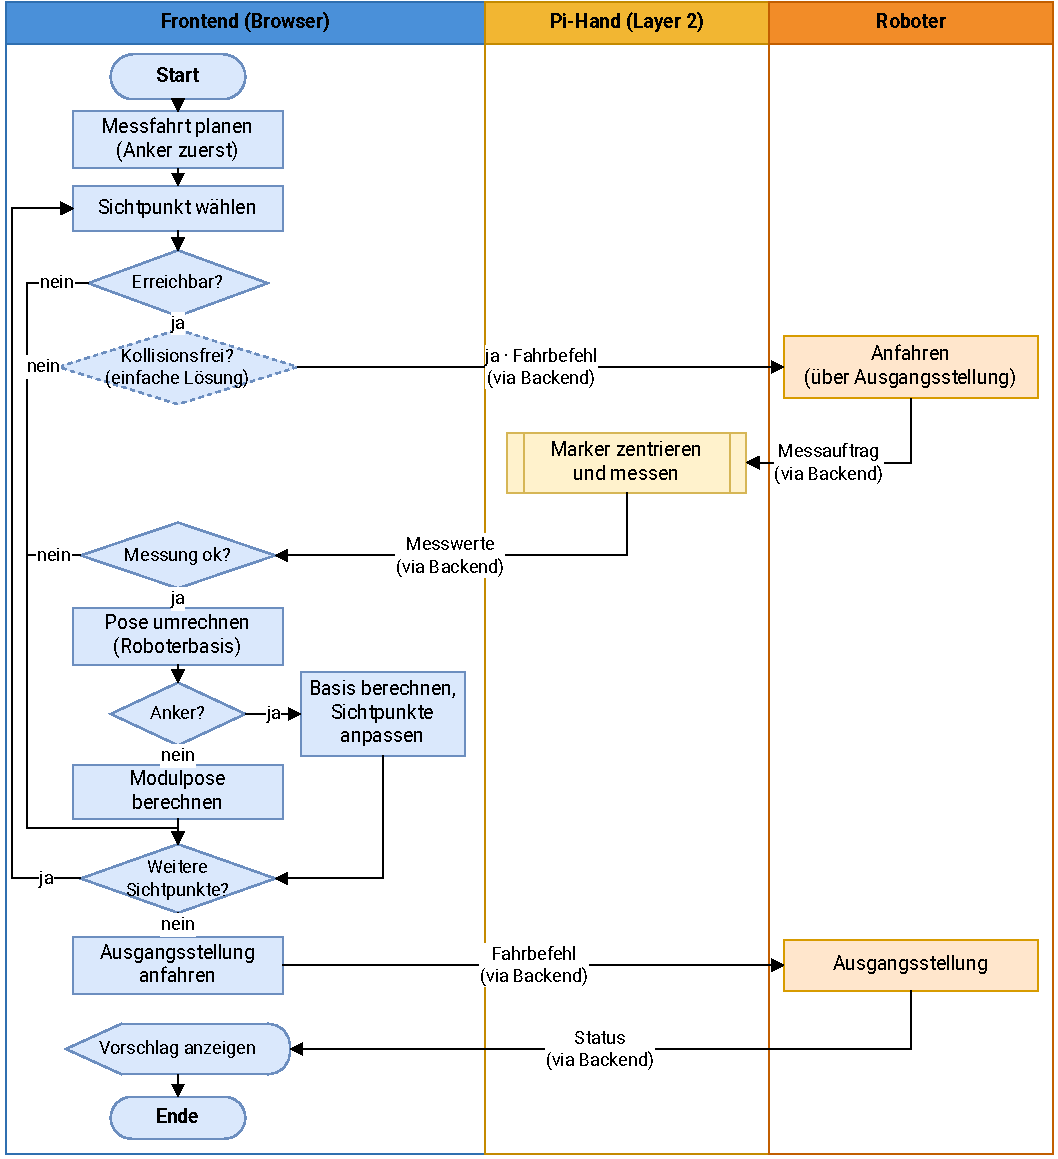
\includegraphics[width=0.85\textwidth]{05_Layer2_Messen_v3.pdf}
    \caption{Ablauf der Layer-2-Messfahrt}
    \label{fig:vs-messfahrt}
\end{figure}

Die Messfahrt beginnt an einem WorldTag in Reichweite des Roboters, dem Anker. Auch die Lage der Roboterbasis im Weltkoordinatensystem stammt zunächst aus Layer~1 und ist damit nur grob bekannt. Die Lage des Ankers im Weltkoordinatensystem ist eingemessen, seine Lage in der Basis liefert Gleichung~\eqref{eq:vs-kette}. Daraus folgt die korrigierte Lage der Basis:
\begin{equation}
    \mathbf{T}_{\mathrm{Welt,Basis}} = \mathbf{T}_{\mathrm{Welt,Anker}} \cdot \mathbf{T}_{\mathrm{Basis,Anker}}^{-1} .
    \label{eq:vs-anker}
\end{equation}
Mit dieser Basis werden die Sichtpunkte der Module neu geplant. Die Module werden danach im selben Bezug gemessen wie die Welt.

Der Sichtpunkt eines ModulTags liegt \SI{35}{\centi\metre} vor dem Tag. In diesem Abstand ist der Tag groß genug im Bild, und die wenigen Zentimeter Abweichung aus Layer~1 bleiben im Bildfeld. Den Anker sieht die Kamera aus etwa \SI{1}{\metre}. Die WorldTags liegen auf dem Boden und die Roboterbasis etwa \SI{1}{\metre} darüber, und mit \SI{200}{\milli\metre} Kantenlänge sind sie aus dieser Entfernung gut zu erkennen. Ist der senkrechte Blick auf einen Tag nicht erreichbar, wird die Ansicht schrittweise zum Roboter hin geneigt und weiter entfernt geplant, mit dem Tag weiterhin in der Bildmitte. Die Drehung der Kamera um ihre Sichtlinie ist frei, genommen wird die erste, die der Arm erreicht.

Jeder Sichtpunkt wird mit einer numerischen inversen Kinematik auf dem URDF-Modell des Roboters gelöst. Eine Lösung gilt, wenn sie das Ziel auf \SI{2}{\milli\metre} und \SI{1}{\degree} genau trifft. Startwert ist die aktuelle Stellung, damit der Arm seine Konfiguration behält. Jede Ansicht wird mit mehreren Drehungen der Kamera um ihre Blickachse und mehreren Startwerten geplant. Vor dem Fahren wird jede Stellung und der Weg dorthin auf Kollision mit dem Wagen und dem Boden geprüft. Der Arm wird dafür als Kette von Kugeln modelliert, die Glieder mit \SI{6}{\centi\metre} und die Hand mit \SI{8}{\centi\metre} Radius, zuzüglich \SI{2}{\centi\metre} Sicherheitsabstand. Der Weg zwischen zwei Stellungen wird so fein abgetastet, dass kein Gelenk mehr als \SI{0,05}{\radian} je Prüfschritt fährt. \Add{[OFFEN: Kollision mit anderen Modulen geprüft?]}

Für jede Modulpose speichert der Zwilling zusätzlich die gemessene Pose des Tags im Basiskoordinatensystem. Anwendungen wie das Ablegen eines Würfels greifen direkt auf diese Messung zu und umgehen damit den Weg über das Weltkoordinatensystem. Die erreichte Genauigkeit zeigt Kapitel~\ref{ch:Verifikation}. \Add{[OFFEN: Dauer einer Messfahrt je Tag]}

 \section{Kommunikation und Integration}
 \label{sec:communikation_intergration}
 Die grundlegende Funktionsweise von OPC UA wurde bereits in Abschnitt~\ref{sec:Kommunikationstechnologien} beschrieben. Für dieses Projekt sind vor allem die Companion Specifications wichtig. Sie legen fest, wie ein bestimmter Gerätetyp seine Daten und Funktionen beschreibt. Für Bildverarbeitungssysteme gibt es OPC UA for Machine Vision. Teil~1 beschreibt, wie ein Bildverarbeitungssystem über eine feste Zustandsmaschine gesteuert wird und wie es seine Ergebnisse bereitstellt \cite{OPC40100-1}. Teil~2 ergänzt Angaben zum Gerät selbst und zu seinem Zustand, zum Beispiel ob es fehlerfrei arbeitet \cite{OPC40100-2}. Unabhängig vom Gerätetyp definiert OPC UA in Part~10 sogenannte Programme. Ein Programm ist ein Ablauf mit festen Zuständen, den ein Client starten, anhalten und zurücksetzen kann. Das Ergebnis liest er danach an einer festen Stelle aus \cite{OPC10000-10}.

Bei der Zusammenarbeit mehrerer Geräte muss die Kommunikationsbeziehung klar geregelt sein. Dafür dient das Backend als Gateway, dieses verbindet sich mit allen OPC-UA-Servern. Das Frontend spricht nur mit dem Backend. So muss der Browser kein OPC UA implementieren und ein Gerät lässt sich austauschen, ohne dass sich am Frontend etwas ändert. Nach einem ähnlichen Prinzip arbeitet ein Aggregation Server. Er fasst mehrere OPC-UA-Server zu einem zusammen, sodass ein Client nur noch eine Adresse kennen muss \cite{Sain2026}. Damit Geräte auch ohne feste Adresse gefunden werden, sieht OPC UA einen Local Discovery Server (LDS) vor. Server melden sich dort an, Clients fragen dort nach. Über die Erweiterung mit Multicast DNS (mDNS) kündigen sich Server zusätzlich selbst im lokalen Netz an \cite{OPC10000-12}.

 abschließend ist festzulegen, welche Daten über die Schnittstelle laufen. OPC UA eignet sich gut für kleine, strukturierte Werte wie Zustände, Befehle und Messergebnisse. Für große Datenmengen wie Bilder oder einen fortlaufenden Videostream ist es nicht gedacht. Über OPC UA werden daher ausschließlich Posen, Statuswerte und Fehlercodes ausgetauscht.

 Jeder Pi betreibt einen eigenen OPC-UA-Server auf Basis der Python-Bibliothek asyncua. Intern bildet der Server das Bildverarbeitungssystem nach Teil~1 der Machine-Vision-Spezifikation ab, mit Zustandsmaschine und Ergebnisverwaltung. Den Gerätezustand meldet er nach Teil~2. Das Backend greift auf diese Struktur aber nicht direkt zu. Als einheitlicher Einstieg dient das Programm nach Part 10. Dieses Programm dient als Wrapper um das Bildverarbeitungssystem und das Backend spricht ausschließlich darüber mit dem Pi. Einen Messauftrag startet es über die Zustandsmaschine des Programms und liest danach das Ergebnis aus. Auch die übrigen Funktionen sind darüber implementiert. So muss das Backend keinen Pi im Detail kennen.

 Ein Ergebnis enthält für jedes erkannte Modul eine Pose. Dazu gehören die Position in Metern, die Orientierung als Quaternion, das Bezugssystem und ein Wert für die Konfidenz. Ein Quaternion beschreibt eine Drehung im Raum mit vier Zahlen, in denen die Drehachse und der Drehwinkel stecken. Es ist mathematisch elegant und numerisch stabil. Im Gegensatz zu Euler-Winkeln hat es keine Sonderstellungen, in denen eine Drehachse verloren geht, und mehrere Drehungen lassen sich einfach miteinander verketten. Neben Rotationsmatrix und Euler-Winkeln ist es deshalb eine der gängigen Formen, Orientierungen zu speichern und auszutauschen \cite{Diebel2006}. Die Ergebnisse werden als JSON-Text übertragen. Fehler meldet der Pi als feste Fehlercodes. Zu jedem Code ist ein deutscher Klartext hinterlegt, den das Frontend dem Bediener direkt anzeigen kann.

 Für das Auffinden der Pis wird die vorhandene Infrastruktur der Zelle genutzen. Beim Start meldet sich jeder Pi beim LDS der Zelle an und erneuert diese Anmeldung regelmäßig, wie es die Spezifikation verlangt \cite{OPC10000-4}. Dadurch nimmt ihn der Aggregation Server der Zelle automatisch auf. Zusätzlich kündigt sich der Pi per mDNS an, sodass ihn das Backend über seine bereits vorhandene mDNS-Suche findet. Nach dem Verbinden sucht das Backend auf jedem Server nach Part-10-Programmen und bindet diese als Gerät ein. Ob es sich um den Decken- oder den Hand-Pi handelt, erkennt das Frontend an der Seriennummer. Neue Geräte lassen sich so nach dem Prinzip Plug and Play einbinden. Nicht nur ein weiterer Pi, sondern jedes Gerät mit einem Part-10-Programm wird ohne Änderung am Frontend erkannt.

 Der Roboter bringt einen eigenen OPC-UA-Server nach der Companion Specification für Robotik mit \cite{OPC40010-1}. Seine Ansteuerung über das Backend sowie Take Control und Sync waren bereits vorhanden und werden unverändert genutzt.

Zusätzlich bietet jeder Pi einen Livestream seiner Kamera an (gestrichelte Linie in Abbildung 4.1). Der Stream gehört nicht zum Messsystem. Er dient nur dazu, das System bei Vorführungen anschaulich zu machen, und läuft unabhängig vom übrigen Ablauf. Weil OPC UA nicht für fortlaufende Bilddaten gedacht ist, wird dafür einen einfachen HTTP-Stream im MJPEG-Format genutzt. Der Browser lädt ihn direkt vom Pi. Damit die Vorschau weder das Netz noch die Pis unnötig belastet, wird sie in geringerer Auflösung übertragen. Die Messung ist davon nicht betroffen, denn sie arbeitet immer mit dem vollen Kamerabild.

 \section{Frontend-Integration in den digitalen Zwilling}
 \label{sec:digitaler_zwilling}
% Notiz aus dem Team (übernommen): Kein Plan was hier rein soll, haben wir bis jetzt kein Digitalen Zwilling erklärt? Dann muss das alles hier gemacht werden. Hier haben wir gefühlt nichts gemacht das gab es schon. Hier gehört die  Erklärung des Modulkatalogs hin (in 4.1 nur kurz eingeführt): Aufbau eines Eintrags (ID, Art, Abmessungen, 3D-Modell, Tags mit Lage am Modul), Welt-Tags mit fester Pose, Roboter mit OPC-UA-Adresse, neues Modul nur per Katalogeintrag ohne Code-Änderung, Bearbeitung im Frontend und Speicherung im Backend. Auch Tag einmessen würde ich als subsection einbauen, würde Meric aber übernehmen
% Abschnitt 4.6: Entwurf erstellt mit Claude Opus 5.5 (Anthropic), siehe KI-Hilfsmittel-Verzeichnis.
Die Messergebnisse werden erst nutzbar, wenn sie im digitalen Zwilling ankommen. Dort wird die Zelle angezeigt, die Messfahrt geplant und der Roboter gesteuert. Dieser Abschnitt beschreibt zunächst den vorhandenen Zwilling und danach, was für die Lokalisierung hinzugekommen ist: der Modulkatalog, das Einmessen der Tags, die Darstellung der Messergebnisse, die Vorschau vor jeder Fahrt und die Bedienung.

\subsection{Ausgangsbasis}
\label{subsec:dz-basis}
Der digitale Zwilling baut auf der Webanwendung WebSkillComposition auf. Sie dient der fähigkeitsbasierten Steuerung von Industrierobotern und besteht aus einem Python-Backend und einem Frontend im Browser. Die Roboter werden als URDF-Modelle in einer 3D-Szene dargestellt, unterstützt sind der FR3, der EVA von Automata und der UR5e. Im Simulationsbetrieb wirken Bewegungen nur auf den Zwilling. Der Bediener stellt die Gelenke direkt ein oder bewegt den Werkzeugpunkt über die inverse Kinematik. Mit Sync übernimmt der Zwilling die Bewegungen des realen Roboters und schickt eigene Bewegungen an ihn zurück. Aktionen wie \texttt{goto} ruft das Backend als Methode oder als Skill des Robotikservers auf, ohne dass das Frontend den Unterschied kennen muss.

Vor diesem Projekt kannte der Zwilling damit den Roboter, aber nicht seine Umgebung. Module, Tische und ihre Lage in der Zelle kamen in der Szene nicht vor. Diese Lücke schließt die Lokalisierung. Sie ist als eigener Funktionsbereich ergänzt und lässt sich vollständig über das vorhandene Web-Frontend bedienen, wie A7 es verlangt.

\subsection{Modulkatalog}
\label{subsec:dz-katalog}
Abschnitt~\ref{sec:gesamtarchitektur} hat den Modulkatalog kurz eingeführt. Er ist die einzige Stelle, an der beschrieben ist, welche Module das System kennt, und Kameras wie Zwilling beziehen ihre Angaben von dort. Stünden diese Angaben an mehreren Stellen, würden sie mit der Zeit auseinanderlaufen. Der Katalog liegt als JSON-Datei im Backend. Das Frontend lädt und speichert ihn über eine HTTP-Schnittstelle, und jede Änderung erhöht seine Revisionsnummer. So ist erkennbar, ob alle Beteiligten mit demselben Stand arbeiten. Tabelle~\ref{tab:dz-katalog} zeigt den Aufbau eines Eintrags.

\begin{table}[htbp]
    \centering
    \caption{Aufbau eines Eintrags im Modulkatalog}
    \label{tab:dz-katalog}
    \begin{tabularx}{\textwidth}{lX}
        \toprule
        \textbf{Angabe} & \textbf{Inhalt} \\
        \midrule
        ID und Name    & eindeutige Kennung und Anzeigename \\
        Art            & Modul, Roboter oder WorldTag \\
        Abmessungen    & Quader um das Modul im Modulkoordinatensystem \\
        3D-Modell      & Datei im Format STL, glTF, DAE oder URDF \\
        Tags           & je Tag ID, Kantenlänge und Lage am Modul, also $\mathbf{T}_{\mathrm{Tag,Modul}}$ aus Gleichung~\eqref{eq:bv-kette} \\
        nur WorldTag   & eingemessene Pose im Weltkoordinatensystem \\
        nur Roboter    & Robotermodell (URDF) und OPC-UA-Adresse des Robotikservers \\
        \bottomrule
    \end{tabularx}
\end{table}

Die drei Arten unterscheiden sich darin, wie ihre Lage entsteht. Ein Modul wird über seine Tags gemessen und in die Szene gestellt. Ein WorldTag hat eine feste, eingemessene Pose und legt das Weltkoordinatensystem fest. Ein Roboter wird wie ein Modul über seinen Tag platziert. Über die OPC-UA-Adresse verbindet der Zwilling ihn zusätzlich mit dem realen Roboter, und das Robotermodell bestimmt, mit welchem URDF-Modell geplant wird.

Ein neues Modul ist damit nur ein neuer Katalogeintrag, Programmcode muss dafür nicht geändert werden (A1). Angelegt und bearbeitet werden die Einträge samt 3D-Modell im Frontend, gespeichert werden sie im Backend. Die Pis erhalten daraus über OPC~UA die Kantenlängen der Tags und die Lage der WorldTags.

Vor dem Speichern prüft der Zwilling jeden Eintrag. Fehler, die ein Modul falsch oder mehrdeutig platzieren würden, verhindern das Speichern. Dazu gehören ein Modul ohne Tag, eine Tag-ID außerhalb der 587~Codes der Familie tag36h11, ein Tag, der schon an einem anderen Modul sitzt, und die ID eines WorldTags an einem Modul. Hinweise lassen das Speichern zu, sollten aber geprüft werden. Ein Beispiel ist ein Tag, dessen Mitte mehr als \SI{1}{\centi\metre} von der Oberfläche des Moduls entfernt liegt. Ein anderes ist eine Tag-Größe, die nicht zu der Größe passt, mit der eine Kamera rechnet.

\subsection{Einmessen der Tags}
\label{subsec:dz-tag-einmessen}
\Add{[OFFEN: Diesen Unterabschnitt schreibt Meric. Ein Entwurf zur Tag-Platzierung auf Modellflächen steht als Kommentar im Quelltext darunter.]}
% Entwurf (Ming, mit Claude Opus 5.5) als Vorlage für Meric:
% Die Lage eines Tags auf seinem Modul wird mit einem eigenen Werkzeug festgelegt. Der Bediener legt den Tag auf eine Fläche des 3D-Modells und gibt die Abstände zu zwei Bezugskanten ein, die er am realen Modul mit dem Lineal misst. Dafür muss der Zwilling die ebenen Flächen eines Modells und ihre Kanten kennen. Ein CAD-Modell besteht jedoch nur aus Dreiecken, oft aus Millionen. Die meisten davon beschreiben gekrümmte Teile. Die Flächen werden deshalb in zwei Schritten gefunden:
% \begin{enumerate}
%     \item \textbf{Ebenen sammeln.} Jedes Dreieck wird nach seiner Normalen und seinem Abstand vom Ursprung einer Ebene zugeordnet, und je Ebene wird die Fläche aufsummiert. Nur Ebenen mit nennenswerter Fläche werden weiter betrachtet.
%     \item \textbf{Flächen und Kanten bilden.} Zusammenhängende Dreiecke einer Ebene bilden eine Fläche. Kanten, die nur zu einem Dreieck gehören, bilden ihren Rand. Der begradigte Rand liefert die Bezugskanten, und wo zwei Kanten sich schneiden, liegt eine Ecke. Bei Tischen aus Aluminiumprofilen ist die Oberfläche durch die Nuten in Streifen geteilt. Lücken bis zur Breite einer Nut werden deshalb überbrückt, sodass die ganze Tischplatte eine Fläche bildet.
% \end{enumerate}
% Mit demselben Werkzeug lässt sich eine Tag-Lage nachträglich prüfen. Es zeigt die Abstände der gemessenen Tag-Mitte zu den Bezugskanten neben den Werten aus dem Katalog an, gemessen in der Ebene des Tags wie mit einem aufgelegten Lineal.

\subsection{Messergebnisse in der Szene}
\label{subsec:dz-szene}
Ein Layer-1-Scan wird vollständig ausgewertet, bevor er die Szene verändert. Der Bediener sieht zuerst, welche Module der Scan platzieren würde, welche WorldTags der Decken-Pi gesehen hat und wo die Kamera steht. Auch der Roboter ist dabei ein Modul mit eigenem Tag. Seine Basis folgt aus der Lage dieses Tags auf seinem URDF-Modell. Ist im Katalog sein Robotikserver hinterlegt, wird der Zwilling mit dem realen Roboter verbunden. Eine Messfahrt lässt sich erst starten, wenn ein solcher Scan übernommen wurde und der Roboter darin platziert und verbunden ist.

Vorwärts- und inverse Kinematik berechnet das Frontend auf demselben URDF-Modell, das auch die Szene zeigt. Was der Bediener sieht, ist damit genau das, womit die Messfahrt geplant wird. Jedes Modul trägt eine Genauigkeitsstufe, die an der Farbe seines Umrisses zu erkennen ist. Nach einem Layer-1-Scan ist es \glqq grob\grqq{}, nach einer übernommenen Layer-2-Messung \glqq genau\grqq{}. Ein Layer-2-Vorschlag zeigt alte und neue Lage nebeneinander, zusammen mit Verschiebung, Drehung und Streuung der Messungen. Wurde die Drehung aus Layer~1 behalten (Abschnitt~\ref{subsec:vs-regelung}), steht das im Vorschlag. Sieht ein neuer Layer-1-Scan ein genau vermessenes Modul mehr als \SI{10}{\centi\metre} oder \SI{10}{\degree} von seiner genauen Lage entfernt, wurde es offenbar verschoben. Seine genaue Lage gilt dann nicht mehr, und es fällt auf \glqq grob\grqq{} zurück.

Abbildung~\ref{fig:dz-ergebnis} zeigt den Weg vom Vorschlag bis zur Zellüberwachung. Das Frontend startet die Überwachung auf dem Decken-Pi und zeigt ihren Alarm an. Noch unbestätigte Änderungen erscheinen sofort, zusammen mit der Zeit bis zur Meldung. Hält der Bediener eine gemeldete Änderung für unerheblich, kann er sie ignorieren. Das aktuelle Bild wird dann zur neuen Referenz. Nach jedem übernommenen Layer-1-Scan wird die Überwachung mit diesem Scan als Referenz neu gestartet.

\begin{figure}[htbp]
    \centering
    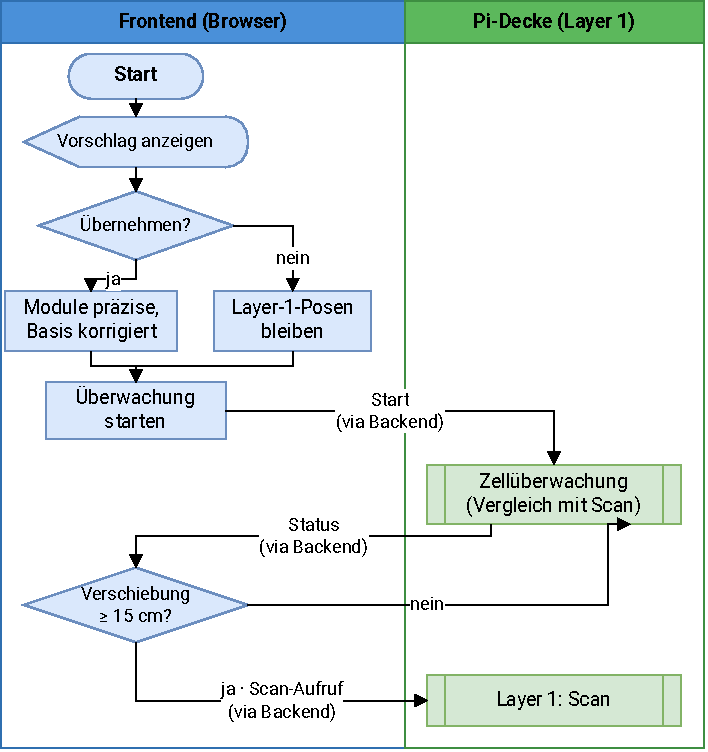
\includegraphics[width=0.55\textwidth]{06_Ergebnis_v3.pdf}
    \caption{Übernahme des Layer-2-Ergebnisses und Zellüberwachung}
    \label{fig:dz-ergebnis}
\end{figure}

\subsection{Vorschau und Fahren}
\label{subsec:dz-fahren}
Bevor sich der reale Roboter bewegt, zeigt der Zwilling, was geschehen wird. Er zeichnet den geplanten Weg mit allen Haltepunkten in die Szene und stellt die Zielstellung als halbtransparenten Roboter dar. Ziele, die nicht erreichbar sind, werden markiert statt angefahren. Erst danach bestätigt der Bediener die Fahrt, und ein Haltbefehl bricht sie jederzeit ab (A6).

Für eine bestätigte Fahrt schaltet der Zwilling Take Control und Sync selbst ein, in der Reihenfolge, in der es auch der Bediener täte. Jeder Schritt wird geprüft und nicht vorausgesetzt: Take Control wartet auf die Antwort des Robotikservers, Sync darauf, dass der Abgleich läuft. Scheitert ein Schritt, nennt die Meldung genau diesen. Nach der Fahrt schaltet der Zwilling nur das wieder aus, was er selbst eingeschaltet hat. Ein Roboter, den der Bediener schon von Hand übernommen hatte, bleibt so in seiner Hand. Ein Fahrbefehl ist eine Bewegung auf Zielwerte der Gelenkwinkel mit einstellbarer Geschwindigkeit. Nach jedem Befehl wartet der Zwilling den Stillstand ab (Abschnitt~\ref{subsec:vs-regelung}).

\subsection{Bedienung}
\label{subsec:dz-bedienung}
Tabelle~\ref{tab:dz-funktionen} listet die Funktionsbereiche, die für die Lokalisierung hinzugekommen sind. Abbildung~\ref{fig:dz-screenshot} zeigt den Zwilling während einer Messfahrt.

\begin{table}[htbp]
    \centering
    \caption{Funktionsbereiche der Lokalisierung im digitalen Zwilling}
    \label{tab:dz-funktionen}
    \begin{tabularx}{\textwidth}{lX}
        \toprule
        \textbf{Bereich} & \textbf{Aufgabe} \\
        \midrule
        Modulkatalog           & Module, Tags, Umrisse und 3D-Modelle anlegen, prüfen und pflegen \\
        Tag-Werkzeuge          & Tags auf Modellflächen platzieren, Tag-Lagen mit dem Lineal prüfen \\
        Layer~1                & Scan auslösen, Ergebnis vorab ansehen und übernehmen, Zellüberwachung starten \\
        Layer~2                & Messfahrt planen und in der Vorschau zeigen, Anker und Module anfahren, Ergebnis als Vorschlag zeigen \\
        Kalibrierung           & Brett für die Deckenkamera führen, Aufnahmeposen der Hand-Auge-Kalibrierung planen und anfahren, Kalibrierung prüfen \\
        Pick-and-Place         & Aufnahme einlernen, Ablage und Rücknahme planen und fahren, Foto zur Auswertung \\
        \bottomrule
    \end{tabularx}
\end{table}

\begin{figure}[htbp]
    \centering
    \fbox{\parbox[c][4.5cm][c]{0.85\textwidth}{\centering\Add{[BILD OFFEN: Bildschirmfoto des digitalen Zwillings mit Zelle, gemessenen Modulen und Layer-2-Fenster]}}}
    \caption{Digitaler Zwilling mit gemessenen Modulen und geplanter Messfahrt}
    \label{fig:dz-screenshot}
\end{figure}

Für den Anwendungsfall Pick-and-Place legt der Roboter einen Würfel auf einem Tisch ab, der nur über die Lokalisierung bekannt ist. Der Ablageort ist relativ zu einem Tag des Tischs festgelegt und wird direkt aus dessen Layer-2-Messung im Basiskoordinatensystem berechnet. Fehlt eine gültige Messung, startet die Ablage nicht. Nach jeder Ablage nimmt die Handkamera ein Foto senkrecht von oben auf, und der Zwilling speichert dazu einen vollständigen Datensatz des Laufs. Die Auswertung folgt in Kapitel~\ref{ch:Verifikation}.

Geometrie und Planung sind als reine Funktionen von der Oberfläche getrennt. Sie sind mit Unit-Tests abgesichert, die ohne Roboter und Kameras laufen. \Add{[OFFEN: Anzahl der Tests zum Abgabestand]}
